% The course-machinery manual. Compiled WITH the machinery it documents: the
% class and packages below are the shipped ones, loaded exactly as a course
% document would load them -- so if the manual builds, the toolkit works.
\documentclass{CourseDocument}

% CourseDocument itself loads Typefaces[osf], Titling, Hyperlinks and
% InstructorNotes. The manual adds the rest of the toolkit so it can DEMONSTRATE
% it, in the same order LectureNotes.cls loads it (the canonical order; see the
% load-order contract in Part 3).
\usepackage{Exercises}
\usepackage{ProblemMeta}
\usepackage{Workspace}
\usepackage{MathStuff}
\usepackage{CourseBoxes}

% Manual-local example machinery (source-plus-rendered blocks). Not shipped.
\usepackage{manual-style}

% Force every content layer ON: the point of the manual is to SHOW solutions,
% hints and instructor notes. In a real course document these are off and
% injected per-view by build-pdfs; see "How to read this manual".
\solutionstrue
\hintstrue

% Solid mode: boxes at natural height, so rendered examples stack normally.
% The default overlay mode (zero-height boxes painting into reserved
% \workspace) is demonstrated -- and explained -- in its own chapter.
\solidboxes

\title{The Course Machinery}
\subtitle{Guide and reference for \texttt{.course-machinery}\\[1ex]
  \normalfont\normalsize\itshape three document classes, the exercise system,
  and the build scripts}

\begin{document}

% The canonical CourseDocument opening (documented in CourseDocument.cls:
% \maketitle runs on the plain page style, the TOC gets its own, and the
% running head starts after) -- the same idiom a syllabus uses.
\maketitle
\pagestyle{toc}
\tableofcontents
\newpage
\pagestyle{myfancy}

\section{How to read this manual}

This manual is compiled \emph{with} the toolkit it documents: its class is the
shipped \file{CourseDocument}, its packages are the shipped ones, and every
rendered example below is typeset by the real machinery at build time. If the
manual builds, the toolkit works.

Examples appear in boxes like this one -- the source on top is the \emph{same
text} that produced the rendered result underneath, so the two can never drift
apart:

\begin{manexample}
A limit shorthand from MathStuff:
$\inflim \frac{1}{n} = 0$.
\end{manexample}

Three things to keep in mind while reading:

\begin{itemize}
  \item \textbf{Every content layer is switched on.} This manual forces
    solutions, hints and (locally) instructor notes to display, because its job
    is to show them. In a real course document these layers are \emph{off}; the
    build script turns them on per view, producing separate student, solutions,
    hints and instructor PDFs from one source. Part 1 explains that model.
  \item \textbf{Counters are live.} A rendered \env{problem} steps the real
    problem counter, so example problems number consecutively through the
    manual, exactly as they would in a course document.
  \item \textbf{Solid mode is active.} Boxes here occupy their natural height.
    The default \emph{overlay} mode -- solution boxes of zero height that paint
    into reserved whitespace so every view has identical page breaks -- has its
    own chapter, and one live demonstration there.
\end{itemize}

Where to start: section~\ref{sec:quickstart} for the shape of a course
repo, then whichever workflow you are sitting down to do. The reference
(Part~\ref{part:reference}) and the architecture notes
(Part~\ref{part:architecture}) are for looking things up later.


\part{Workflows}
\section{Quickstart: anatomy of a course repo}\label{sec:quickstart}

A course lives in one repository, organised by topic, with this machinery in
a hidden subdirectory. The demo course (\file{course-demo}) is the
reference layout:

\begin{manexsource}
course-demo/
  .course-machinery/        the toolkit (classes, packages, scripts)
  .course-machinery-local/  machinery for THIS course, shared across files
    books.tex               the book registry: every book the course names,
                            with its title and URLs. Loaded into EVERY
                            document, whole
    textbook.tex            the text layer: what a book NAMES things -- the
    openstax.tex            vocabulary, which is exclusive. The first is the
                            course default; a second file is a second book,
                            chosen per document with \usetext
  .MIRRORDIR                optional PDF mirror destination
  derivatives/              a topic (a course has several, same shape)
    problems/               problem bank: one problem per file
    lectures/               LectureNotes masters (+ .latexmkrc, which puts both
                            machinery folders on TEXINPUTS; build-pdfs installs
                            it, one identical copy per build directory)
    facts/                  fact bank: one tagged snippet per file
    images/
  _assessment/              Assessment masters (+ .latexmkrc)
  _syllabus/                CourseDocument masters (+ .latexmkrc)
\end{manexsource}

Three document classes cover every document a course produces -- when you
sit down to write, the only decision is which one:

\begin{itemize}
  \item \file{Assessment} -- anything graded or handed in: tests, finals,
    quizzes, homework (\texttt{[noid]}), worksheets. Clear and standard;
    nothing fancy. Section~\ref{sec:assessments}.
  \item \file{LectureNotes} -- lecture handouts, with a projector view for
    the room. Big type, board space, imported examples.
    Section~\ref{sec:lectures}.
  \item \file{CourseDocument} -- prose documents: syllabus, TA info,
    policies. Coloured headings, TOC, reading measure.
    Section~\ref{sec:prose-documents}.
\end{itemize}

Underneath them, shared packages supply the content machinery -- the same
problem environments, boxes, whitespace commands and fonts everywhere, so
one problem file moves freely between a test and a lecture. You rarely load
any of them yourself; the class does (Part~\ref{part:reference} documents
each).

\subsection{The wiring}

Documents name their class plainly -- \cs{documentclass}\texttt
{\{LectureNotes\}} -- and never spell out where it lives. The
\file{.latexmkrc} in each \file{.tex}-holding directory makes that work: it
walks up to the repo root and puts \file{.course-machinery//} and
\file{.course-machinery-local/} on \env{TEXINPUTS} for that build --- the
two tiers of machinery that are shared across files. Everything else a
document loads sits beside it and is found in the cwd
(section~\ref{sec:extending}). The copies are identical, and you never plant
them yourself: latexmk reads only the rc in its startup directory and never
walks up, so \file{build-pdfs} installs one in each source's directory before
compiling. Creating a new topic folder takes no setup at all.

Cross-file inclusion uses the \file{import} package's relative paths, so one
source serves every consumer. A lecture and the quiz pull the \emph{same}
\file{power-rule-basic.tex} by the path each needs -- \file{../problems/}
beside it, \file{../derivatives/problems/} from the repo root -- and any
images that file loads resolve against the \emph{file's own} directory.

The course-wide content files are two, and the split between them is the
one thing worth learning early. \file{.course-machinery-local/textbook.tex}
is the \emph{text layer}: what the book \emph{names} things --- the result
boxes it uses (APEX's ``Key Idea''), the noun lectures call an example.
That is \emph{exclusive}, since a document cannot use two vocabularies at
once, so \cs{usetext} picks exactly one.
\file{.course-machinery-local/books.tex} is the \emph{book registry}:
each book's title, publisher and URLs. That is not exclusive at all --- a
syllabus names every book the course uses --- so it is loaded into every
document, whole.

Masters \cs{input} neither --- both are found by name and loaded
automatically, so a lecture may sit at any depth and a new master cannot
forget them. Section~\ref{sec:extending} explains the one-question test for
what belongs there, and why the text layer is guarded. Which \emph{section}
of the book a given lecture covers is declared in that lecture, not here
(section~\ref{sec:ref-textref}).

\subsection{The five-minute loop}

Day to day, the toolkit is a three-step loop:

\begin{enumerate}
  \item \textbf{Write or find problems.} One file per problem in a topic's
    \file{problems/}, tagged; \texttt{find-problems -{}-topic ...} to
    rummage (sections \ref{sec:problem-files}, \ref{sec:build-and-find}).
  \item \textbf{Assemble a document.} A master imports problems (with
    points, on a test; as examples, in a lecture) and declares its views
    in the \texttt{\%! views:} comment.
  \item \textbf{Build.} \texttt{build-pdfs} in the document's directory
    compiles everything there -- student PDF plus each declared view,
    routed to the synced mirror if one is configured
    (section~\ref{sec:build-and-find}).
\end{enumerate}

The rest of Part~1 walks these in order; Part~\ref{part:reference} is the
per-file reference; Part~\ref{part:architecture} explains the architecture
-- the load-order contract, the view/layer model, and how to extend the
vocabulary -- for the day you want to change the machinery itself.

\section{Authoring a problem file}\label{sec:problem-files}

The problem bank is the heart of the system: \emph{one problem per file}, no
preamble, sitting in a topic's \file{problems/} folder. The same file is pulled
into an assessment as a graded question, into a lecture as a worked example, and
into a check-in as a flashcard exercise -- the file itself never changes, only
the import site decides how it appears. Two rules follow from that:

\begin{itemize}
  \item \textbf{A problem file is context-neutral.} It names no label
    (``Q''\,/\,``Example''), no number, and no point value. The consuming class
    supplies the label and number style; the import site supplies the points.
  \item \textbf{A problem file carries what is intrinsically its own}: the
    statement, its hint and solution, and its metadata (topics, tags,
    difficulty, source). Those belong to the problem forever, wherever it is
    used.
\end{itemize}

This intrinsic/extrinsic split is load-bearing. Points are \emph{extrinsic} --
the same problem is worth 5 on one test and 7 on another -- so points are given
where the problem is imported (section~\ref{sec:assessments}), and are
deliberately \emph{not} a metadata field.

\subsection{Anatomy of a problem file}

A complete file, exactly as it sits in the bank:

\begin{manexample}
\ProblemMeta{
  topics     = {differentiation, power-rule},
  tags       = {polynomial, routine},
  difficulty = {basic},
  source     = {own},
}
\begin{problem}
  Differentiate $f(x) = 3x^{4} - 5x^{2} + 2$.
\end{problem}
\begin{hint}
  Differentiate term by term.
\end{hint}
\begin{solution}
  $f'(x) = 12x^{3} - 10x$.
\end{solution}
\end{manexample}

Note what rendered: the metadata block typeset \emph{nothing} (it is
store-only), the problem numbered itself, and -- because this manual forces all
layers on -- the hint and solution both display. In a student build both
disappear without a trace.

To start a new problem, copy an existing file: \file{derivatives/problems/}
in the demo course repo holds one build-tested file of every type.

\subsection{The metadata block}\label{sec:problemmeta}

\cs{ProblemMeta} exists so that ``which problems do I have about the chain
rule?'' is answerable \emph{without running LaTeX} -- nothing has \cs{input}
those files at the moment you are deciding what goes on the test. The
companion script \file{find-problems} answers it by reading the block straight
off disk (section~\ref{sec:find-problems-taste}).

That design puts one discipline on the author -- the block is parsed
\emph{textually}, line by line:

\begin{itemize}
  \item \textbf{One key per line, values braced}, as in the example above. A
    block reflowed onto a single line still \emph{compiles} fine, but the
    problem silently vanishes from the script's index -- the one way to get the
    two readers out of step.
  \item \textbf{Write \texttt{\char`\\\#} for \texttt{\#}} (LaTeX requires it;
    the script strips the backslash back out when reporting, so
    \texttt{source = \{Stewart 3.1 \char`\\\#7\}} reports as
    \texttt{Stewart 3.1 \#7}).
\end{itemize}

The recognised keys are \env{topics}, \env{tags}, \env{difficulty},
\env{source}, and \env{id}. On the LaTeX side they are validated but discarded
-- a mistyped key (\env{topic} for \env{topics}) errors at compile time, so
typos cannot silently un-index a problem. Before inventing a new tag, run
\texttt{find-problems -{}-vocab} to see the vocabulary already in use, and reuse
it.

The block is also optional insurance, not a hard dependency: the exercise
system compiles problem files with or without \file{ProblemMeta.sty} loaded (a
stub swallows the block), so tagging can be adopted -- or abandoned --
without touching the bank.

\subsection{Problems, hints, and solutions}

\env{problem} numbers itself on a document-wide counter and is
cross-referenceable. How the heading \emph{looks} -- ``Problem 7.'' here,
``Q\,7'' with margin marks on a test, a run-in ``Example.'' in lecture notes --
is the consuming class's business, through presentation hooks
(section~\ref{sec:hooks}); the numbering and points bookkeeping stay in the
environment, so no restyle can break the count.

\env{hint} and \env{solution} ride along in the same file, each gated by its
own layer:

\begin{itemize}
  \item \textbf{A solution is the answer key} -- shown only in a solutions
    build, set in the green box you saw above. \env{solution}\texttt{[notitle]}
    drops the corner tab, leaving a bare box.
  \item \textbf{A hint is student-facing help} -- shown only in a hints build,
    as a light run-in (deliberately plainer than a solution: a nudge, not the
    answer). It sits inline where written, not collected at the end.
\end{itemize}

The two layers are independent: a hints build is not a solutions build, and a
per-import key can force one problem's hint on or off against the document
toggle (section~\ref{sec:assessments}).

\subsection{Dependent parts in one file: \env{qparts}}

When parts genuinely depend on each other -- one stem, sub-questions (a), (b),
(c) -- they are \emph{one} problem and belong in \emph{one} file, with the
parts marked by \cs{qpart}:

\begin{manexample}
\begin{problem}
  Evaluate.
  \begin{qparts}
    \qpart Find $\lzoo{x}{x^{2}e^{x}}$.
    \begin{solution}[notitle]
      $2x\,e^{x} + x^{2}e^{x} = x\,e^{x}(x+2)$.
    \end{solution}
    \qpart Find $\lzoo{x}{x^{3}e^{x}}$.
  \end{qparts}
\end{problem}
\end{manexample}

Each part letters itself, and a solution (or hint) can follow its own
\cs{qpart}. Per-part points and per-part workspace are supplied at the import
site, for example \texttt{points=\{2,1\}} and \texttt{workspaces=\{4,4\}} --
keeping even part-level grading extrinsic (section~\ref{sec:assessments}).

The other thing people call ``parts'' -- \emph{independent} problems grouped
under a shared instruction (``Evaluate the following:'') -- is not this. Those
stay atomic one-problem files and are grouped at assembly time with
\env{problemgroup} (section~\ref{sec:assessments}).

\subsection{Multiple choice}

An MC question is \emph{not} a separate problem type: it is a normal
\env{problem} whose body carries a \env{choices} list -- so it numbers, grades,
tags and imports exactly like everything else. Mark the key with the optional
argument:

\begin{manexample}
\begin{problem}
  What is the domain of $f(x)=\dfrac{\sqrt{x+1}}{x-7}$?
  \begin{choices}
    \choice{$\{x : x \ge -1\}$}
    \choice{$\{x : x > -1\}$}
    \choice[correct]{$\{x : x \ge -1,\ x \ne 7\}$}
    \choice{$\{x : x > -1,\ x \ne 7\}$}
  \end{choices}
\end{problem}
\end{manexample}

The key is boxed \emph{only} in a solutions build (the green cue above -- gated
by the same toggle as \env{solution}, so the answer never leaks into a student
copy), and swapping which option is correct is an in-place edit. Marking
several options \texttt{[correct]} makes a select-all-that-apply.

One environment, three layouts:

\begin{manexample}
Is $f(x) = x^{3}$ even, odd, both, or neither?
\begin{choices}[onepar]
  \choice{Even}
  \choice[correct]{Odd}
  \choice{Both}
  \choice{Neither}
\end{choices}
\end{manexample}

\begin{itemize}
  \item \emph{(default)} -- one option per line, for long options;
  \item \texttt{[onepar]} -- inline, for short options as above;
  \item \texttt{[grid]} -- a grid, \cs{ChoicesGridCols} wide (default 2),
    row-major.
\end{itemize}

For a grid of \emph{graphs}, \cs{graphchoice}\texttt{[correct]\{FILE\}} is a
\cs{choice} that sizes its image to the column and sets the letter beside it.
This manual has no image files, so the grid below is source-only; the live
version is \file{mc-graph-grid.tex} in the demo repo:

\begin{manexsource}
\begin{problem}
  The graph of $y = f(x)$ has a horizontal tangent at $x = 1$. Which of
  the following could be the graph of $y = f'(x)$?
  \begin{choices}[grid]
    \graphchoice{../images/cubic}
    \graphchoice[correct]{../images/tangent}
    \graphchoice{../images/parabola}
    \graphchoice{../images/step}
  \end{choices}
\end{problem}
\end{manexsource}

\subsection{Matching}

A matching question is likewise a normal \env{problem}. Left items carry the
answer key intrinsically -- each names its match in the optional argument, shown
(green-boxed) only in a solutions build:

\begin{manexample}
Match each function with its derivative.
\begin{matching}
  \leftitem[B]{$\sin x$}
  \leftitem[C]{$\cos x$}
  \leftitem[A]{$\tan x$}
  \rightcolumn
  \rightitem{$\sec^{2} x$}
  \rightitem{$\cos x$}
  \rightitem{$-\sin x$}
  \rightitem{$\sec x \tan x$}
\end{matching}
\end{manexample}

Left items letter in lowercase roman, right items in uppercase alphabetic --
two visibly different systems, so ``match [i] with [C]'' can never be
misread. The columns may have different lengths (distractors on the right, as
above), and \cs{rightcolumn} splits them with a wide gap for students to draw
their connecting lines in. Graph items reuse the \cs{graphchoice} sizing:
\cs{leftgraph}\texttt{[X]\{FILE\}} / \cs{rightgraph}\texttt{\{FILE\}} put
graphs in either column. The demo's \file{match-graphs-phrases.tex} keeps the
graphs on the \emph{right} so the answer key rides the roomy text column rather
than a column-width image; \file{match-trig-derivatives.tex} matches text to
text. There are deliberately no drawn answer arrows -- the inline key on the
left item is the answer, and skipping arrows keeps the system TikZ-free.

\subsection{Finding problems in the bank}\label{sec:find-problems-taste}

The payoff for the metadata discipline -- from anywhere in the course repo:

\begin{manexsource}
$ find-problems --topic chain-rule --difficulty basic
$ find-problems --vocab      # the tag vocabulary in use, with counts
$ find-problems --untagged   # the tagging backlog
$ find-problems --import     # print matches as paste-ready \import lines
\end{manexsource}

Filters combine (AND), match case-insensitively as regular expressions, and
never run LaTeX. The full command reference is in
section~\ref{sec:build-and-find}.

\section{Writing a lecture}\label{sec:lectures}

A lecture is a \file{LectureNotes} document. The class comes in two sizes from
one source: the default 14\,pt \emph{handout} (printed or posted for students),
and a 17\,pt \emph{projector} copy for the room, built automatically as a view
(section~\ref{sec:build-and-find}). A typical master, from the demo repo's
\file{derivatives/lectures/1.1-IntroToDerivatives.tex}:

\begin{manexsource}
%! views: projector, instructor
\documentclass{LectureNotes}
\collapseworkspace

% Per-course text-result vocabulary (e.g. APEX's "Key Idea").
\input{../../course-vocab}

\begin{document}
\section*{Introduction to Derivatives}
...
\end{document}
\end{manexsource}

Three preamble notes. The \texttt{\%! views:} comment declares which extra PDFs
the build script produces (here a projector copy and an instructor copy). The
\cs{collapseworkspace} switch selects natural-height boxes -- the right mode when the
notes carry no reserved whitespace; see section~\ref{sec:overlay} for the
whole story. And \file{course-vocab.tex} is \cs{input} \emph{in the preamble}
(its box declarations must run before the document starts), via a relative
path from the repo root -- section~\ref{sec:extending} explains what belongs
in that file.

\subsection{Text results: boxes with declared numbers}

\file{CourseBoxes} provides the boxed results -- and its numbering model is
the one thing to internalise: box numbers are \emph{declared, not counted}.
You type the number, matching the course text, and \cs{label}/\cs{ref} work as
usual:

\begin{manexample}
\begin{definition}{2.1.1}[Derivative]\label{def:deriv}
  The derivative of $f$ at $x$ is
  $f'(x) = \lim_{h \to 0} \frac{f(x+h) - f(x)}{h}$,
  provided the limit exists.
\end{definition}

\begin{theorem}{2.1.4}[Power Rule]\label{thm:power}
  For any real constant $n$, $\lzo{x}\,x^{n} = n\,x^{n-1}$.
\end{theorem}

Theorem~\ref{thm:power} rests on Definition~\ref{def:deriv}; the
text's 2.1.2 and 2.1.3 are simply skipped.
\end{manexample}

Because nothing is counted, the notes mirror the textbook's own numbering and
may skip freely -- the gap above is the feature, not a bug. Keeping LaTeX's
automatic counters aligned with a textbook means fighting them document-wide;
declaring the number is one argument at the call site.
Section~\ref{sec:extending} covers the mechanism and how to add
course-specific vocabulary (\env{keyidea}, \env{axiom}, \dots).

The universal environments, always available: \env{theorem},
\env{proposition}, \env{lemma}, \env{corollary}, \env{definition},
\env{example}, and \env{remark}, all with the same
\texttt{\{number\}[optional name]} signature.

\subsection{Pedagogical asides}

Asides are the \emph{author's} voice -- unnumbered, never referenced, and
deliberately not \cs{label}-able (they are commentary, not results). Two of
the five, live:

\begin{manexample}
\begin{caution}
  The Power Rule is for a \emph{variable base, constant
  exponent}. It does not apply to $2^{x}$.
\end{caution}

\begin{tip}[surviving]
  Remember: $\frac{1}{a+b} \neq \frac{1}{a} + \frac{1}{b}$.
\end{tip}
\end{manexample}

The full set: \env{caution}, \env{takeaway}, \env{yourturn}, \env{prepwork},
and \env{tip} -- where \env{tip} takes an optional audience tier,
\texttt{[surviving]} or \texttt{[thriving]}, that stamps the box for the
struggling or the confident reader respectively (a bare \env{tip} is for
everyone).

\subsection{Importing problems as examples}

The same problem files that grade as ``Q'' on a test
(section~\ref{sec:assessments}) read as worked examples in notes. The class
renders an imported problem with a run-in \textbf{Example.} heading --
unnumbered by default, because the default example is improvised board work,
not a text citation:

\begin{manexsource}
\importproblem{../problems/}{power-rule-basic.tex}
% -> "Example.  Differentiate f(x) = ..."

\importproblem[number={2.1.8}, desc={from APEX}]
  {../problems/}{power-rule-basic.tex}
% -> "Example 2.1.8 (from APEX).  Differentiate f(x) = ..."
\end{manexsource}

The \texttt{number=} key sets a \emph{literal} display number (typically the
textbook's -- the same declared-number philosophy as the boxes; a \cs{ref} to
the problem reads ``2.1.8'' too), and \texttt{desc=} adds a parenthetical
note. Points keys are simply ignored in notes -- the same import line can
move between a test and a lecture unchanged.

Two more import forms round out the lecture repertoire:

\begin{itemize}
  \item \cs{importcheckin} (same arguments as \cs{importproblem}) wraps an
    imported multiple-choice problem in a framed ``CHECK IN:'' box with
    coloured A--E flashcard labels -- the in-class poll format. Same file,
    third appearance.
  \item \env{problemgroup} assembles independent one-file problems under a
    shared stem; in notes the stem stays an unnumbered ``Example.''\ and the
    members letter themselves (a), (b) (see section~\ref{sec:assessments}
    for the graded version).
\end{itemize}

The ``Example'' noun itself is a per-course choice (texts say Example /
Exercise / Problem): redefine \cs{NotesProblemLabelWord} in
\file{course-vocab.tex} and every lecture follows, without touching the fixed
``Q'' on assessments.

\subsection{Instructor-only annotations}

Lectures carry notes-to-self and co-teacher asides that students must never
see. Three shapes, all in slate and all invisible outside an instructor build
(the flag is flipped locally here to show them):

\begin{manexample}
\instructornotestrue
Some lecture prose.
\InstructorInline{Most will try to memorise this before
understanding it -- resist that.}

\begin{InstructorBox}[marking]
  Budget a full board example on expanding-then-cancelling
  before the Power Rule.
\end{InstructorBox}
\end{manexample}

The \cs{InstructorInline} note is a run-in aside in the paragraph flow;
\env{InstructorBox} is a side-barred block (the rotated word says \emph{note},
or \emph{marking} with the optional argument); \cs{InstructorMargin} drops a
bold sans note in the margin (not shown live -- this manual's example boxes
sit too far from the page margin for it to land sensibly). In an instructor
build, every page also gets a page-edge frame reading \emph{Instructor copy}
-- the copy identifies itself even from a glance at a single page.

\subsection{Board space and the projector copy}

\cs{workspace}\texttt{[N]} reserves $N$ lines of handwriting room -- in
lectures, space to improvise at the board while students follow on the
handout. It is the same command assessments use for answer space;
section~\ref{sec:overlay} explains it (and how solutions can \emph{overlay}
that space without moving anything).

The projector view needs no source changes at all: \texttt{\%! views:
projector} makes the build script produce \file{...-PROJECTOR.pdf} alongside
the handout -- 17\,pt type, tighter margins, no page number, and a grey
back-to-top arrow in the footer (the room copy is scrolled, not paged). Two
class behaviours worth knowing: every \cs{subsection} starts a fresh page (a
lecture section is a screenful), and only \cs{section} is numbered.

\section{Building an assessment}\label{sec:assessments}

An assessment -- test, final, quiz, homework -- is an \file{Assessment}
document: an assembly file that sets up a cover, then imports problems from
the bank with points attached. The skeleton, modelled on the demo's
\file{_assessment/test.tex}:

\begin{manexsource}
%! views: solutions, instructor
\documentclass[12pt,thursday,automatch]{Assessment}
\assessmentsetup{
  course = {MATH 101},
  term   = {Fall 2026},
  name   = {Term Test 1},
  date   = {16 Oct},
  instructions = {
    \textbf{\sffamily Instructions:}
    \begin{itemize}[nosep]
      \item \printtotalpoints\ points.
      \item Closed book. No calculators.
      \item Show all work for full marks.
  \end{itemize}},
}
\begin{document}
\AssessmentTitle
\newpage
\importproblem[points=5]
  {../derivatives/problems/}{chain-rule.tex}
\workspace[5]
...
\end{document}
\end{manexsource}

The class renders questions as ``Q\,$N$'' hung in the \emph{left} margin with
their point marks ``($N$ pts)'' in the \emph{right} margin -- numbers left,
marks right, so standalone questions and lettered group parts drop their marks
into the same rail. None of that appears in this manual's examples (which
render with the neutral ``Problem $N$.''\ style); build the demo's
\file{test.tex} to see the real thing.

\subsection{Class options}

\begin{itemize}
  \item \texttt{[noid]} -- for documents that collect no student identity:
    homework, in-class worksheets, MC practice. Drops the NAME/ID box and the
    deep scanner top margin. The \emph{default} is the fully-furnished
    identified exam, on purpose: forgetting \texttt{[noid]} merely
    over-furnishes homework with an unused ID box, whereas the opposite
    default could ship a real exam with no ID box at all -- the safe mistake
    is the easy one to make.
  \item \texttt{[automatch]} -- for Crowdmark's automatic name matching:
    keeps the deep top margin (the QR code still lands there) but replaces
    the NAME/ID box with a blank mid-cover band (9--18\,cm down the page, per
    spec) where students write their identity for the scanner.
  \item \texttt{[tuesday]} / \texttt{[thursday]} -- a framed day box beside
    the title: TUE on the \emph{left}, THU on the \emph{right}, so two
    section piles sort at a glance by which side the box sits on, without
    reading a word.
  \item \texttt{[legalpaper]} -- legal stock; the margins stay absolute, so
    the extra three inches become writing room.
  \item Stock \file{article} options pass through (\texttt{[12pt]},
    \texttt{[twoside]}, \dots).
\end{itemize}

About that deep top margin: Crowdmark stamps a QR code into the top band of
every page at upload, so the band stays clear of content throughout, and the
cover's NAME/ID box is lifted up \emph{into} it, beside where the QR lands.

\subsection{The cover}

\cs{assessmentsetup} takes the five fields you saw above -- \env{course},
\env{term}, \env{name}, \env{date}, \env{instructions} -- every one optional;
an unset field prints nothing, brackets and all. Anything else an exam cover
might say (time allowed, formula-sheet note, coverage) is just prose in
\env{instructions}, which needs no dedicated keys. \cs{AssessmentTitle} then
emits the cover: NAME/ID box, centred title, instructions.

Note what is \emph{not} a field: the point total. Write
\cs{printtotalpoints} in the instructions (as above) and the printed total is
summed from the imported problems themselves -- it can never disagree with
the paper. (Both this total and the ``Page $N$ of $M$'' footer are two-pass
values: a first compile shows \texttt{??}, and the build's latexmk rerun
settles it.)

In a solutions build, the cover also stamps itself
{\sffamily\bfseries\color{SolutionColor}SOLUTIONS} -- the answer key
announces itself.

\subsection{Points at the import site}

Points are attached where a problem is imported, never stored in the problem
file (section~\ref{sec:problem-files}). The grammar, in increasing order of
ceremony:

\begin{manexsource}
\importproblem[5]{DIR}{FILE}          % shorthand: points=5
\importproblem[points=5]{DIR}{FILE}   % the same, spelt out
\importproblem[points=2*]{DIR}{FILE}  % announced BONUS: off the total
\importproblem[points=5, nocount]{DIR}{FILE}  % quiet: off the total
\importproblem[points={2,1*}, workspaces={4,4}]{DIR}{FILE}
                                      % per-part (a qparts file)
\importproblem[pointseach=2]{DIR}{FILE}   % broadcast to every part
\importproblem[points=5, hint]{DIR}{FILE} % force this hint ON
\end{manexsource}

\begin{itemize}
  \item \textbf{Values are integers} -- the total accumulator and the
    singular/plural logic both require it; \texttt{points=2.5} errors.
  \item \textbf{The \texttt{*} suffix means announced bonus}: the value is
    shown (a bonus \emph{is} worth $N$ if earned), labelled \emph{bonus} in
    the margin, and kept out of \cs{printtotalpoints}. In a per-part list,
    star just the bonus part: \texttt{points=\{2,3,1*\}} makes only part (c)
    bonus.
  \item \textbf{\texttt{nocount} is the quiet off-books case} -- marker
    unchanged, total untouched. Its main use is choose-$N$-of-$M$ accounting,
    where \env{problemchoice} below applies it for you.
  \item \textbf{One seam to know}: the lone-integer shorthand only fires when
    the whole option is one integer, so \texttt{[5, hint]} errors -- write
    \texttt{[points=5, hint]}.
  \item \texttt{hint} / \texttt{nohint} force one problem's hint on or off
    against the document toggle -- a worked example on a test, or a hint
    withheld in an otherwise-hinted homework.
\end{itemize}

\subsection{Grouping: \env{problemgroup} and \env{problemchoice}}

\env{problemgroup} assembles \emph{independent} one-file problems into one
numbered question with lettered parts -- the parts stay atomic files in the
bank, and each import inside carries its own points, exactly as anywhere
else:

\begin{manexsource}
\begin{problemgroup}{Evaluate}
  \importproblem[points=5, hint]
    {../derivatives/problems/}{quotient-rule.tex}
  \workspace[3]
  \importproblem[5]
    {../derivatives/problems/}{second-derivative.tex}
  \workspace[2]
\end{problemgroup}
\end{manexsource}

This renders as ``Q\,$N$.\ Evaluate'' with parts (a), (b); a \cs{ref} to a
part reads ``$N$(a)''. To \cs{label} the \emph{group}, put the label just
inside \env{problemgroup}, before the first part -- after \cs{end} it would
catch the last part instead. (Genuinely dependent sub-questions are one file
with \env{qparts}, section~\ref{sec:problem-files} -- import that file here
like any other.)

\env{problemchoice} is the choose-$N$-of-$M$ wrapper:

\begin{manexsource}
\begin{problemchoice}[select=2, points=5]
  \importproblem[]
    {../derivatives/problems/}{mc-domain.tex}
  \FreshPage
  \importproblem[]
    {../derivatives/problems/}{mc-tangent-slope.tex}
  \FreshPage
  \importproblem[]
    {../derivatives/problems/}{mc-select-all.tex}
\end{problemchoice}
\end{manexsource}

Each member question repeats the generated instruction (``Answer any two of
Questions $N$--$M$.''\ -- page-break safe), every member shows the shared
per-question value, and the total counts it $\text{select} \times
\text{points}$ once, not per member. Members therefore carry no
\texttt{points=} of their own (one that does triggers a warning, since it
would silently diverge from the shared value).

\texttt{instruction=} says \emph{where} that sentence appears, and the
default is the block above: \texttt{each}. Repeating it earns its keep when
the choice is one block among required questions -- a student meeting Q8
alone still learns that it is one of a choice. It is noise when the
\emph{whole paper} is one choice, where the sentence is really a fact about
the paper: then set \texttt{instruction=first} to announce the run once, or
\texttt{instruction=none} and say it in the cover instructions.

\begin{manexsource}
\begin{problemchoice}[select=5, points=6, instruction=none]
\end{manexsource}

\noindent
Nothing checks that the paper says it somewhere -- this package cannot read
your cover. Both \cs{label}s are still dropped in every mode, so a cover line
can name the range itself with \cs{ref}\texttt{\{pc@1@first\}} and
\cs{ref}\texttt{\{pc@1@last\}} (the digit is the group's number, counting
from one).

\subsection{Answer space and page furniture}

\cs{workspace}\texttt{[N]} reserves $N$ lines of handwriting after a question
(also \texttt{[halfpage]}, \texttt{[fullpage]}, or \cs{workspace*} to fill
the rest of the page); \cs{FreshPage} is a collapsible page break;
\cs{FreshPage}\texttt{[blank]} and \texttt{[watermark]} emit a dedicated
blank page, the latter stamped ``Blank page for extra work.'' All of this is
Workspace machinery with one deep design idea -- reserved space that
solutions can paint into without moving a single page break -- explained in
section~\ref{sec:overlay}.

The class's own page furniture is minimal and load-bearing: a ``Page $N$ of
$M$'' footer on every page (a student can check the stapled packet is
complete at a glance) and no running head.

\subsection{Views of one assessment}

With \texttt{\%! views: solutions, instructor} in the magic comment, the
demo's \file{test.tex} builds three PDFs: the student paper, an answer key
(\file{-SOLUTIONS}), and the staff bundle (\file{-INSTRUCTOR}: solutions +
hints + instructor notes, inside the page-edge \emph{Instructor copy} frame).
Under the default overlay mode all three have \emph{identical page breaks} --
the whole point of section~\ref{sec:overlay}. (Add \texttt{hints} to the list
-- as the demo's \file{quiz.tex} does -- for a fourth, student-facing
\file{-HINTS} copy.) Build mechanics are in section~\ref{sec:build-and-find}.

\subsection{Printing the cover on its own}

A test's first page is the one page you may want to print by itself --- on
heavier paper, or in a different quantity from the paper behind it. Adding
\texttt{\%! coverpage: yes} to the magic comment writes
\file{test_COVERPAGE.pdf} beside \file{test.pdf}: page~1 of the finished
test, nothing else. It is taken from the student build only, since a
solutions or instructor cover is the same sheet of paper.

Note \emph{finished}. The obvious way to do this would be a page-selection
package in the preamble, and it does not work here, for a reason worth
knowing because it applies to anything that stops a run early. The cover's
own numbers are two-pass values: \cs{printtotalpoints} is a
\texttt{totcount} sum written to the \file{.aux} at \cs{end\{document\}} and
read back on the next run, and the footer's ``Page 1 of $M$'' is
\cs{pageref\{LastPage\}}. The package for the job, \texttt{pagesel},
suppresses the \file{.aux} outright and aborts the job after the last
selected page --- so the run never reaches the point where the total is
written, and the cover prints the \emph{wrong} number of points. Cutting
page~1 out of a normally-built PDF has no such failure mode: the document
compiled exactly as it always does, and the page is the page.

\section{Prose documents}\label{sec:prose-documents}

Syllabi, TA information sheets, course policies -- continuous prose rather
than problems -- are \file{CourseDocument} documents. It is the ``designed''
class of the three: coloured headings, a titled cover, a table of contents,
and a text measure tuned for reading. (This manual is itself a
CourseDocument.) The demo repo's \file{_syllabus/syllabus.tex}:

\begin{manexsource}
%! views: instructor
\documentclass[11pt]{CourseDocument}

\title{\course{101} --- Syllabus}
\subtitle{%
  Fall 2026, University of New Brunswick \\[1ex]
  \normalfont\normalsize\itshape Sections FR01 and FR02.
}

\begin{document}

\maketitle
\pagestyle{toc}
\tableofcontents

\newpage
\pagestyle{myfancy}

In \course[MATH]{1013} we will be investigating...

\end{document}
\end{manexsource}

That opening sequence is the documented idiom, worth copying verbatim.
\cs{maketitle} runs while the page style is still \texttt{plain}, so the
title page stays bare; the contents page then opts into \texttt{toc}
(footer page number only); and \texttt{myfancy} -- a small-caps running
head with the current section, page number in the footer -- starts with the
body. Neither named style activates itself: each document chooses when.

The pieces in play:

\begin{itemize}
  \item \cs{title} and \cs{subtitle} feed a shared title block that also
    stamps \emph{Updated \textnormal{(date, time)}} -- these documents are
    living and revised mid-term, and the stamp says which printing is
    current. The subtitle's second line above shows the usual trick for a
    quieter sub-subtitle: reset the font inline.
  \item \cs{course}\texttt{[MATH]\{1013\}} sets a course designation in the
    body serif with lining numerals, tied so it cannot break across lines --
    consistent wherever it appears, prose or title. The bracket defaults to
    the course's own prefix, so \cs{course}\texttt{\{101\}} works too.
  \item Headings, the title block and internal links all carry the course
    identity colour -- named \emph{once} (\env{CourseIdentity}, a mahogany)
    and used unmodified, so restyling a course document is a one-line
    change. Deliberately \emph{not} green: green means ``solutions, not for
    students'' everywhere else in the toolkit, so a student-facing document
    must not read as green.
  \item \texttt{[legalpaper]} is available, as on assessments; stock
    \file{article} options pass through.
\end{itemize}

Body text in this class uses old-style figures -- the numerals with
ascenders and descenders you see in this manual's prose -- because these
documents are continuous reading. Dates, office numbers and the like sit
quietly in the text; \cs{liningnums}\texttt{\{2026\}} forces lining figures
where a number should read as data, and math and \cs{course} numerals stay
lining automatically. The full figure policy lives with
\file{Typefaces.sty} (section~\ref{sec:ref-typefaces}).

Not every prose document wants them, though. A syllabus is only half
continuous reading: the other half is \emph{data} scanned rather than
read -- test dates, room numbers, section codes, percentage weights --
and a page of those in old-style figures reads as restless. When
\cs{liningnums} starts appearing more often than not, stop reaching for
it and set the class option instead:

\begin{manexsource}
\documentclass[11pt,lining]{CourseDocument}
\end{manexsource}

\noindent It is a class option and not something a preamble can do for
itself, because Typefaces is loaded during \cs{documentclass} -- by the
time a document could pass it an option, it is already in. The two
choices are exclusive: name \texttt{lining} and the class passes exactly
that to Typefaces in place of \texttt{osf}.

Two things CourseDocument deliberately lacks: the exercise system (a
syllabus imports no problems -- the class loads no Exercises/Workspace
machinery), and any use of \cs{workspace}. It \emph{does} carry the
instructor-notes layer, so a syllabus can hold staff-only annotations --
office-hour strategy, grading-scheme rationale -- and ship an
\file{-INSTRUCTOR} view like any other document
(section~\ref{sec:build-and-find}).

\subsection{Passages}\label{sec:ch5-passages}

A \textbf{passage} is prose that belongs to the author rather than to the
course: why the subject is worth the effort, how marking works, what makes a
solution readable. Because it is shared across courses it lives in its own
content repository, mounted beside the topic submodules and reached by
relative path --- it is content, not a tier (see the architecture chapter).

The reason this is a command rather than a bare \cs{input} is \textbf{heading
level}. The same passage is a \cs{section} of one document and a
\cs{subsection} of another, and a passage carrying headings of its own has to
move with its title. So the file is written at its \emph{natural} depth ---
\cs{PassageTitle} for its own title, plain \cs{subsection} for anything
inside it --- and the importing document says where that lands:

\begin{manexsource}
% teaching/passages/why-learn-math.tex
\PassageMeta{
  title = {Why Learn Math?},
  label = {sec:whylearnmath},
}
\PassageTitle
Mathematics is beautiful, powerful, and useful.
\end{manexsource}

\begin{manexsource}
\importpassage{../teaching/passages/}{why-learn-math.tex}
\importpassage[level=subsection]{../teaching/passages/}{why-learn-math.tex}
\end{manexsource}

\noindent \cs{PassageTitle} takes \emph{no arguments}. Its title and its
\cs{label} both come from the \cs{PassageMeta} block above it --- the same block
\file{find-passages} reads off disk (section~\ref{sec:ref-passagemeta}). The
label names the passage's own idea, so it belongs to the passage rather than to
whichever document imports it.

Unlike \cs{ProblemMeta} and \cs{FactMeta}, which are validated and thrown away,
this block is read at build time, so it is not optional: a passage with no
\env{title} is an error rather than an empty heading.

The shift is three \cs{let}s inside a group, run top-down so each captures the
still-original meaning of the level below. \cs{PassageTitle} then needs no
special case --- it is \cs{section}, already pointed at the right target ---
and \cs{label}, \cs{ref}, starred forms and table-of-contents entries keep
working because these are the real sectioning commands.

\textbf{One level of headroom, and deeper is an error.} This class styles
three heading levels and \cs{paragraph} is not among them, so \texttt{level}
accepts \texttt{section} (the default) or \texttt{subsection} and refuses
anything further rather than degrading silently. A passage may therefore carry
one rank of headings below its title and no more. In practice that is the
constraint that decides how a passage is cut: a body of prose with three
ranks is two passages, not one.

A passage needing a number the course owns names a macro --- say
\cs{PointsPerQuestion} --- and lets the course define it in its own
\file{courseinfo.sty}. There is no machinery for that on purpose: a course
that imports a passage without defining what it needs gets an
undefined-control-sequence error, which is the loud failure wanted. Writing
\emph{around} a parameter travels further than introducing one.

\section{Building and finding: the scripts}\label{sec:build-and-find}

One executable builds; a small family searches. \file{build-pdfs} compiles
course documents (with their views, and with output routed where you want
it). The searchers are per-kind faces of one shared engine:
\file{find-problems} searches the problem bank, \file{find-facts} the fact bank
and \file{find-passages} the passage bank -- each a two-line shim that hands the
right \texttt{-{}-kind} to \file{find-meta}, where all the real logic lives once
-- and their interactive twins \file{pick-problems} / \file{pick-facts} /
\file{pick-passages} (shims over \file{pick-meta} the same way) thread those
searches through fzf. Every one of them prints its full reference with
\texttt{-{}-help}.

\subsection{\texorpdfstring{\texttt{build-pdfs}}{build-pdfs}}

\begin{manexsource}
$ build-pdfs              # compile every .tex in this directory
$ build-pdfs test.tex     # just this one (FILE.tex -> FILE.pdf)
\end{manexsource}

The script runs latexmk from each file's own directory, so relative imports
resolve and the directory's \file{.latexmkrc} puts the machinery on
\env{TEXINPUTS}. It installs that \file{.latexmkrc} on the way in: latexmk
reads only the rc in its startup directory and never walks up, so before
compiling, \file{build-pdfs} copies \file{latexmkrc-shared} from the machinery
into the source's directory whenever the file there is missing or out of date.
A new topic folder therefore needs no setup, and an edit to the master reaches
every course on its next build. A copy whose \texttt{managed by build-pdfs}
marker line has been deleted counts as hand-tuned and is never overwritten.
Auxiliary files (\file{.aux}, \file{.log}, \dots) go to a
per-directory folder under \file{~/.cache/latexmk/} -- they clutter neither
the repo nor the output directory -- keyed by the directory's repo-relative
path, so two topics' same-named \file{problems/} folders never share
latexmk state.

\subsubsection{Views: one source, several PDFs}

A magic comment in a source's \emph{leading} comment block (it must precede
\cs{documentclass}) requests extra PDFs:

\begin{manexsource}
%! views: solutions, hints, instructor
\documentclass[12pt,thursday]{Assessment}
\end{manexsource}

Four views are wired, each injecting a layer definition ahead of the source
so the call site needs no class option:

\begin{itemize}
  \item \env{solutions} $\to$ \file{FILE-SOLUTIONS.pdf}: defines
    \cs{ShowSolutions}, so \env{solution} bodies and the boxed MC keys
    print.
  \item \env{hints} $\to$ \file{FILE-HINTS.pdf}: defines \cs{ShowHints}.
    Independent of solutions -- a hint is student-facing help, so list both
    views if you want both PDFs.
  \item \env{projector} $\to$ \file{FILE-PROJECTOR.pdf}: defines
    \cs{ProjectorView}, switching \file{LectureNotes} to the 17\,pt room
    copy.
  \item \env{instructor} $\to$ \file{FILE-INSTRUCTOR.pdf}: the staff
    bundle -- solutions $+$ hints $+$ instructor notes, inside the
    page-edge frame. A view is a \emph{bundle of layers}; the instructor
    copy is the staff copy (TAs get it too -- there is no separate marker
    tier).
\end{itemize}

An unrecognised view name warns and is skipped; the student PDF always
builds. Under the default overlay mode, every view of a document has
identical page breaks (section~\ref{sec:overlay}).

\subsubsection{Where the PDFs go}

The output mirror is one \file{.MIRRORDIR} file, found by walking up from the
build directory to the nearest ancestor that holds one (the repo top level,
the way \file{.latexmkrc} finds the machinery). Its first bare line names a
base directory (leading \texttt{\~{}} expanded) that \emph{mirrors the repo
tree}: a source built in \file{REPO/integrals/lectures} ships its PDF to
\file{BASE/integrals/lectures}. The mirror subdirectory is created if absent,
but the base itself must exist -- if the cloud drive is unmounted, the script
warns and builds locally rather than scattering a stray tree. By default the
PDF goes \emph{straight there}, with no local copy; add a line reading
\texttt{BOTH} to build locally \emph{and} copy. Blank and \texttt{\#}-comment
lines are ignored; the base path and the \texttt{BOTH} keyword may come in
either order. A nearer \file{.MIRRORDIR} in a subdirectory wins, letting a
subtree mirror somewhere else. With no \file{.MIRRORDIR} above it at all, the PDF
lands next to its source.

\file{SAMPLE-MIRRORDIR}, shipped with the machinery, is the commented template --
copy it to \file{.MIRRORDIR} and uncomment. \file{.MIRRORDIR} is meant to be
git-ignored: each machine points its own way.

\paragraph{Routing a view to a named folder.}
Sometimes one view of a document belongs somewhere else too -- the instructor
copy of a test in a folder shared with TAs, say, while the rest of the build
still mirrors to your private cloud. Add \texttt{LABEL: path} lines to
\file{.MIRRORDIR} and tag the view with a matching \texttt{:LABEL} suffix in the
magic comment:

\begin{manexsource}
%! views: solutions, instructor:TA-dir
\end{manexsource}

\noindent That drops \file{FILE-INSTRUCTOR.pdf}, flat, into the directory
\texttt{TA-dir:} names \emph{in addition} to the mirror; \env{solutions} still
goes only to the mirror. The labelled directory must already exist (a missing
label or directory warns and skips just that extra copy -- the build still
succeeds and still mirrors). Because the source names only a \emph{label} and
the git-ignored \file{.MIRRORDIR} maps it to a path, no machine-specific path ever
enters a tracked source. The pseudo-view \env{default} names the base (student)
PDF itself, so \texttt{default:LABEL} routes it the same way; a bare
\env{default} is a harmless no-op.

Routing decides \emph{where} a view goes, not \emph{when} it is released: if
you would rather TAs not see solutions until after the assessment, point the
label at a private staging folder and copy across by hand at release time --
\file{build-pdfs} deliberately knows nothing about dates.

\subsection{\texorpdfstring{\texttt{find-problems} / \texttt{find-facts} /
  \texttt{find-passages}}{find-problems / find-facts / find-passages}}

\begin{manexsource}
$ find-problems [--topic PAT] [--type PAT] [--difficulty PAT]
                [--source PAT] [--untagged] [--vocab] [--import]
                [--tsv] [PATH ...]
$ find-facts    [--topic PAT] [--source PAT] [--untagged] [--vocab]
                [--import] [--tsv] [PATH ...]
$ find-passages [--audience PAT] [--untagged] [--vocab]
                [--import] [--tsv] [PATH ...]
\end{manexsource}

Reads the \cs{ProblemMeta} (resp.\ \cs{FactMeta}, \cs{PassageMeta}) block off
every \file{.tex} file under each \env{PATH} (default: the current directory,
recursively) and reports the matches -- without running LaTeX, which is the
point (section~\ref{sec:problem-files}). With no filters, it lists every
file that has a block. The kind fixes the block macro it reads, the
\cs{importproblem}~/ \cs{importfact}~/ \cs{importpassage} lines it emits, and
the filter set -- facts carry no \env{type} or \env{difficulty}, and a passage is
searched by \env{audience} alone, so the three have four, two and one filters
respectively. Everything below holds for all three.

One difference is worth stating here rather than leaving to be discovered:
\file{find-passages} accepts no \texttt{-{}-with}. A passage has no injectable
keys, because the only option \cs{importpassage} takes is \env{level}, and where
a passage's natural depth lands belongs to the importing document rather than to
the passage (section~\ref{sec:ref-passagemeta}). Emitted passage lines are
therefore always bare. The passage bank also sits in a sibling submodule rather
than a directory of the course, so give it as an operand ---
\texttt{find-passages teaching/passages} --- or a bare run from the course root
will walk everything else too.

Filters combine with AND. \env{PAT} is an extended regular
expression matched case-insensitively against each comma-separated item, so
\texttt{-{}-topic power} finds \texttt{power-rule} and
\texttt{-{}-topic '\^{}power-rule\$'} matches exactly. A filter on a key a
file does not set never matches -- \texttt{-{}-difficulty basic} will not
sweep in untagged files.

Four modes round it out:

\begin{itemize}
  \item \texttt{-{}-vocab} ignores the filters and prints the type and topic
    vocabulary in use, with counts -- the antidote to a bank where half the
    problems say \emph{integration} and half say \emph{integrals}. Read it
    before inventing a type.
  \item \texttt{-{}-untagged} inverts: files with \emph{no} metadata block
    at all -- the tagging backlog.
  \item \texttt{-{}-import} prints the matches as paste-ready
    \cs{importproblem} (or \cs{importfact}) lines. Two opt-in modifiers
    refine the output:
    \texttt{-{}-with LIST} injects a comma subset of the injectable keys as
    options where a file carries them -- \env{number} and \env{name} for a
    problem; for a fact also \env{kind} and \env{name}, which choose and
    title the box it is wrapped in (\env{points} stays manual --
    it is extrinsic) -- and \texttt{-{}-from DIR} rewrites each line's directory
    argument relative to \env{DIR}, the importing document's folder, so the
    pasted line needs no \texttt{../} hand-fixing.
  \item \texttt{-{}-tsv} prints one tab-separated row per match (path, then the
    metadata) -- the machine-readable feed behind the picker below. An operand
    may now be a single \file{.tex} file, not just a directory, so a picker can
    ask \texttt{-{}-import} about exactly the files it selected.
\end{itemize}

The parser is textual and deliberately simple, which is where the
one-key-per-line discipline of section~\ref{sec:problem-files} comes from:
a reflowed block still compiles, but this script no longer sees it.

\subsection{Picking from a bank interactively}

\file{pick-problems} (and \file{pick-facts} / \file{pick-passages}, identically)
threads those two
machine modes through
\href{https://github.com/junegunn/fzf}{fzf}: it feeds \texttt{-{}-tsv} into the
picker (fuzzy-search the metadata, \file{bat}-preview the \file{.tex},
multi-select with Tab), then pipes the chosen files back through
\texttt{-{}-import} so the accepted set comes out as \cs{importproblem} (or
\cs{importfact}, \cs{importpassage}) lines on
standard output. Its \texttt{-{}-from} and any \file{find-problems} filters pass
straight through, e.g.\ \texttt{pick-problems -{}-from \_assessment -{}-type
multiple-choice derivatives/}. The Vim commands \texttt{:ImportProblem}
(\texttt{<Space>ip}), \texttt{:ImportFact} (\texttt{<Space>if}) and
\texttt{:ImportPassage} (\texttt{<Space>ig}) are the same
pipeline, inserting the lines at the cursor
with \texttt{-{}-from} pinned to the buffer's own directory -- so picking a
problem while writing an assessment drops in a ready line, needing only its
\env{points}, and picking a passage drops in one needing nothing at all.

Two things about picking \emph{passages} in particular. The emitted lines are
separated by a blank line, matching how every call site writes them, which makes
each one a paragraph object --- and that matters because fzf returns a
multi-selection in \emph{input} order, not the order you ticked them, while a
passage's position in a document can be load-bearing wherever one passage refers
to another. So reorder after pasting: \texttt{dap}, \texttt{p}. Second, \env{level}\texttt{=subsection} is
always added by hand and is always safe to try: \file{CourseDocument} refuses a
shift that would push a heading past \cs{subsubsection}, loudly, at build time.

\section{The overlay/solid contract}\label{sec:overlay}

This chapter explains the deepest design idea in the toolkit -- why a
solutions copy can show every answer without moving a single page break --
and the one switch that controls it.

\subsection{Reserved space: \cs{workspace}}

Assessments and lectures need copious blank room for handwriting, which is
not the LaTeX norm. \cs{workspace} reserves it \emph{explicitly and visibly
in the source}, as a leaf command between content (never a wrapper around
it), so the source stays readable and the space can be tuned in the editor:

\begin{manexsource}
\workspace            % 8 lines (the default)
\workspace[12]        % 12 lines
\workspace[halfpage]  % about half the text block
\workspace[fullpage]  % the whole text block
\workspace*           % fill to the bottom of this page
\end{manexsource}

The unit is a \emph{line of handwriting} (\cs{HandwritingLine}, about
0.9\,cm) because ``about ten lines'' is how you actually think about writing
room -- centimetres are not. Retune \cs{HandwritingLine} once and
every line-count workspace follows.

One deliberate simplicity: a workspace is plain vertical space, with
\emph{no carry-over}. If it exceeds the room left on the page, the overflow
is dropped and the next content starts the next page -- the gap does not
reappear overleaf. The rare page where that matters is re-spaced by hand,
rather than letting a half-page gap silently wander onto the next page. (A
consequence: like any top-of-page glue, a workspace at the very top of a
page is discarded -- put content above it, or use \cs{workspace*}.)

\cs{FreshPage} completes the spacing toolkit with collapsible page breaks:
bare \cs{FreshPage} breaks to a fresh page that content then flows onto;
\cs{FreshPage}\texttt{[blank]} ships a dedicated empty page;
\texttt{[watermark]} stamps that page with a faint diagonal ``Blank page for
extra work.'' Plain \cs{newpage} remains untouched, for the rare break that
must never collapse.

\subsection{Overlay mode: the default}

Here is the contract. In the default \emph{overlay} mode, the gated boxes --
\env{solution} and \env{InstructorBox} -- render at \textbf{zero height},
painting \emph{downward into the workspace reserved below them} instead of
displacing anything. The reserved space is identical in every build, so:

\begin{center}
  \emph{the solutions or instructor copy is a pixel-perfect overlay\\
  of the student copy -- same layout, same page breaks, same page count.}
\end{center}

That is why the demo's \file{test.tex} can ship three view PDFs
(section~\ref{sec:assessments}) whose page numbers always agree: page 9 of
the answer key \emph{is} page 9 of the student paper, with answers painted
into its blank space. A quick check after any layout change: a source's
views must all have the same page count. If they differ, something has broken the
contract.

Seeing it live -- this example flips the manual back to overlay mode
locally. The solution box adds no height of its own; it simply paints into
the four workspace lines that follow, exactly where a student would write:

\begin{manexample}
\preserveworkspace
\begin{problem}
  Differentiate $h(x) = x^{5}$.
\end{problem}
\begin{solution}[notitle]
  $h'(x) = 5x^{4}$.
\end{solution}
\workspace[4]
\end{manexample}

In the student build the same four lines are simply blank. Two consequences
follow, both intentional:

\begin{itemize}
  \item \textbf{A solution taller than its workspace overprints the content
    below it.} That collision is the alarm -- it says \emph{leave more room
    for this answer} -- not a bug. Fix it by growing the workspace, never by
    shrinking the answer.
  \item \textbf{Hints are not overlays.} A hint is student-facing help that
    should push content down normally in its build -- it participates in
    layout, unlike the answer key painted over blank space.
\end{itemize}

\subsection{Space the key reclaims: \env{studentonly}}

Some of the room an answer needs is already on the page, spent on something
only the student uses -- most often an empty grid to sketch on, which the key
reprints blank and then draws the real graph underneath. \env{studentonly}
hands that room back:

\begin{manexsource}
\begin{problem}
  Sketch the graph of $f$.
  \begin{solution}          % FIRST: it paints downward
    ...prose, and the graph drawn on a grid...
  \end{solution}
  \begin{studentonly}       % its space is kept, its ink dropped
    \PWgrid{}
  \end{studentonly}
\end{problem}
\workspace[10]
\end{manexsource}

The student copy prints the body; the key prints an empty box of exactly the
same height, so the contract above is untouched -- same page breaks, same page
count -- and the solution now has that height \emph{plus} the workspace to
paint into. Adopting it therefore never makes a previously adequate
\cs{workspace} too small. Under \cs{collapseworkspace} the block vanishes
entirely, like every other reservation.

\textbf{The solution must come first.} A solution written \emph{after} the
block starts below the reclaimed space and paints into the workspace instead,
leaving a blank gap where the grid was. Nothing can detect which you meant, so
nothing warns: the key just looks wrong. Note also that the body is measured
by typesetting it, and in the key that box is then discarded -- so keep
\cs{label}s out of a \env{studentonly} body.

\subsection{Solid mode: the compact answer key}

Sometimes the spaced layout is wrong: an answer-key handout to post online,
or lecture notes (this manual runs in solid mode too). One preamble switch:

\begin{manexsource}
\collapseworkspace  % boxes at natural height; workspace and
                    % \FreshPage collapse to nothing
\preserveworkspace  % back to the default overlay mode
\end{manexsource}

Under \cs{collapseworkspace} the boxes carry their own height and \emph{all} the
reserved room -- every \cs{workspace}, every \cs{FreshPage} break and blank
page -- collapses to nothing: the same source becomes a compact document
with answers inline. The collapse happens only under this explicit,
document-wide switch, never silently per-build; within one mode, every view
of a document lays out identically.

A document may keep \cs{preserveworkspace} written out in its preamble even
though it is the default -- a visible declaration of which mode the document
is in, and a smoke test that the switch pair round-trips.


\part{Reference}\label{part:reference}
\section{Assessment.cls}\label{sec:ref-assessment}

The graded-document class: tests, finals, quizzes, homework, worksheets.
Article-based. Loads Exercises, ProblemMeta, Workspace, Typefaces (lining
figures), MathStuff and InstructorNotes; deliberately \emph{not} Titling --
an assessment opens with \cs{AssessmentTitle}, a different artefact from a
styled title. Every page carries a ``Page $N$ of $M$'' footer (two-pass via
\file{lastpage}) and no running head. The text block stays wide, near
article's stock margins: an exam is not continuous prose, so the room goes
to the student's writing, not to a reading measure. Workflow:
section~\ref{sec:assessments}.

\subsection*{Class options}

\begin{center}
\begin{tabular}{@{}l p{0.62\linewidth}@{}}
\texttt{noid} & no student identity collected (homework, worksheets, MC
  practice): drops the NAME/ID box and the deep scanner top margin.\\
\texttt{automatch} & Crowdmark auto-matching: keeps the deep top margin,
  replaces the NAME/ID box with a blank 9--18\,cm mid-cover band.\\
\texttt{tuesday}, \texttt{thursday} & framed day box beside the title, TUE
  left / THU right -- sort two section piles by sight.\\
\texttt{legalpaper} & legal stock; absolute margins, so the extra height is
  writing room.\\
\emph{(other)} & forwarded to \file{article} (\texttt{12pt},
  \texttt{twoside}, \dots).\\
\end{tabular}
\end{center}

The default (no options) is the fully-furnished identified exam --
forgetting an option over-furnishes homework harmlessly, never under-equips
an exam.

\subsection*{Commands}

\begin{center}
\begin{tabular}{@{}l p{0.55\linewidth}@{}}
\cs{assessmentsetup}\texttt{\{...\}} & keyval cover setter: \env{course},
  \env{term}, \env{name}, \env{date}, \env{instructions}; all optional,
  unset fields vanish cleanly.\\
\cs{AssessmentTitle} & emits the cover: NAME/ID box (unless suppressed),
  centred title, instructions; adds a \emph{SOLUTIONS} stamp in a solutions
  build.\\
\cs{BonusMarksOnTop} & bonus margin block as ``(N pts)'' over rule over
  ``bonus'' (the default).\\
\cs{BonusLabelOnTop} & the flip: ``BONUS'' over rule over ``(N pts)''.\\
\cs{BonusMarginLabel}, \cs{BonusMarginRule} & reword the bonus label /
  restyle the divider rule.\\
\cs{ExamTopMargin} & the deep-top length (3.7\,cm), single-sourced for
  geometry and the \texttt{[automatch]} band; rarely touched.\\
\end{tabular}
\end{center}

\subsection*{Presentation choices}

The class overrides the Exercises hooks (section~\ref{sec:hooks}) to the
exam look: questions render as \textbf{Q$N$} hung in the left margin
(\cs{ProblemLabelWord} is \texttt{Q}; \cs{ProblemNumberText} is the tight
``Q$N$'', no space), and every scored item drops its ``($N$ pts)'' mark
into the right margin rail (\cs{ProblemPointsFormat} via \cs{marginnote}) --
numbers left, marks right, so standalone questions and lettered group parts
line up in the same rails. Bonus items stack their mark and label in that
same right rail (\cs{ProblemBonusPointsFormat}). \texttt{number=} and
\texttt{desc=} import keys are ignored: an exam owns its numbering and does
not annotate its questions.

One geometry fact worth knowing rather than rediscovering: the deep
3.7\,cm top margin exists because Crowdmark stamps a QR code into the top
band of \emph{every} page at upload -- interior pages keep the band empty,
and the cover lifts its NAME/ID box up into it, beside the QR.

\section{LectureNotes.cls}\label{sec:ref-lecturenotes}

The lecture class: handouts and their projector twin, from one source.
Based on \file{extarticle} for the large sizes -- 14\,pt handout, 17\,pt
projector. Loads Exercises, ProblemMeta, Workspace, Typefaces (lining),
MathStuff, Titling, Hyperlinks, CourseBoxes and InstructorNotes -- the full
stack. Workflow: section~\ref{sec:lectures}.

\subsection*{Class options}

\begin{center}
\begin{tabularx}{\linewidth}{@{}l Y@{}}
\texttt{projector} & the in-room copy: 17\,pt, tighter top margin, no
  marginpar column, no page number, and the text block sitting left of
  centre (same width, shifted -- see below).
  Normally you never write it -- the build's \env{projector} view injects
  \cs{ProjectorView} and the class switches by itself.\\
\emph{(other)} & forwarded to \file{extarticle}.\\
\end{tabularx}
\end{center}

\subsection*{Commands and hooks}

\begin{center}
\begin{tabularx}{\linewidth}{@{}l Y@{}}
\cs{NotesProblemLabelWord} & the noun imported problems render as
  (default \emph{Example}); redefine per \emph{text}, in
  \file{.textbook/textbook.tex}. Routed into \cs{ProblemLabelWord} so a
  shared text layer cannot disturb Assessment's fixed ``Q''.\\
\cs{lecturetoc} & the lecture's table of contents. Document-called, not
  class-emitted: a short lecture wants none, and only you know which those
  are. Put it straight after \cs{booksection} (lectures have no title
  block). See ``The contents list'' below.\\
\cs{CourseBoxTocEntry} & CourseBoxes' contents hook, rendered here. Renew it
  to change what an entry says.\\
\cs{booksection}, \cs{lecturetitle} & the lecture's title and, for
  \cs{booksection}, the section of the book it covers (with an optional
  \texttt{link=} to that section's page). Supplied by TextRef
  (section~\ref{sec:ref-textref}); the class renders it as the running
  head.\\
\end{tabularx}
\end{center}

\subsection*{Presentation choices}

Imported problems render with a run-in bold heading, unnumbered by default:
\textbf{Example.}\ -- plus the literal \texttt{number=} and parenthetical
\texttt{name=} if the import supplied them (``Example 2.1.8
(differentiating a polynomial).'').\ The problem counter still steps invisibly, so cross-references
stay sound. The \env{problemgroup} stem takes the same unnumbered form.
Points keys are ignored -- notes are ungraded.

Other deliberate class behaviour:

\begin{itemize}
  \item \cs{subsectionbreak} is \cs{clearpage}: every subsection starts a
    fresh page (a lecture subsection is a screenful/boardful).
  \item Only \cs{section} is numbered (\env{secnumdepth} 1); the TOC shows
    three levels.
  \item Paragraph spacing is airier than the parskip default
    (\texttt{skip=1em}) -- room to annotate, legible from the back row.
  \item The running head is the lecture's \cs{booksection} coordinate
    (linked if the book is online), on every page \emph{including} the
    projector copy -- a scrolled
    document is where persistent orientation is worth most. It carries a
    rule, which disappears along with the head if the lecture declares no
    coordinate. Page \emph{numbers} are the opposite case: the handout has a
    centred one, the projector copy none (it is never collated, so a number
    is noise); the projector foot is simply empty.
  \item The projector text block is shifted left of centre
    (\texttt{hmarginratio=\{3:7\}}, so the left margin is 60\% of the centred
    one and the rest falls to the right). Its \emph{width} is the same measure
    as everywhere else -- this moves the block, it does not reflow it. The
    reason is the room: presenting from a tablet puts the app's tool bar down
    the right edge of the screen, over the projected text.
  \item Headings and links stay black: lectures sit with assessments on
    the ``clear, not fancy'' side; colour belongs to CourseDocument.
\end{itemize}

\subsection*{The contents list}

A lecture's contents list is \emph{not} mostly sections -- most lectures
have none. It is mostly the things that actually structure the hour, and it
is assembled from three sources:

\begin{itemize}
  \item every CourseBoxes \textbf{text result} -- definitions, theorems,
    facts, examples, and whatever else the text layer declares -- via
    \cs{CourseBoxTocEntry}. \textbf{Asides never appear}, and not by a list
    of exceptions: they are a different factory, so the exclusion cannot
    drift when a text layer adds a name.
  \item every \textbf{top-level imported problem}, through the same
    renderer, so ``Example 2.1.8'' and ``Definition 2.1.1'' cannot end up
    formatted differently. Parts inside a \env{problemgroup} and check-ins
    stay out for free -- neither reaches the heading hook.
  \item a \env{problemgroup}, \emph{if} it was given a \texttt{name=}. The
    group's stem is a sentence and reads badly in a list, so the name is what
    gets listed; without one the group stays out, since a bare ``Example''
    would be indistinguishable from any other.
  \item \cs{section}/\cs{subsection}, when a lecture uses them.
\end{itemize}

Entries read \emph{Kind number (name)}, dropping whatever is absent:
``Definition 2.1.1 (Derivative)'', ``Example 2.1.5'', ``Theorem (Product,
Quotient, and Chain Rules)''.

Two deliberate presentation choices:

\begin{itemize}
  \item \textbf{Flat, with the typeface carrying the hierarchy.}
    Indentation implies structure; in a sectionless lecture there is none to
    imply, and indenting every result would push the list right for nothing.
    So all levels sit at one margin and sans-bold (headings, echoing the
    page) separates from serif roman (results).
  \item \textbf{Page numbers on the handout only.} The projector copy prints
    no page numbers anywhere, so a page column there would point at numbers
    the reader cannot see. Its entries are hyperlinks instead -- black, so
    they read as plain text and behave as taps.
\end{itemize}

\section{CourseDocument.cls}\label{sec:ref-coursedocument}

The prose class: syllabus, TA information, policies -- and this manual.
Article-based. Loads Typefaces \texttt{[osf]} by default (the only class
with old-style body figures; \texttt{[lining]} opts out), Titling,
Hyperlinks, InstructorNotes and \file{enumitem} (tunable lists --- a policy
document is more list than prose); no
exercise machinery (a syllabus imports no problems -- add the packages in
the preamble if a prose document ever needs them, as this manual does).
Workflow: section~\ref{sec:prose-documents}.

\subsection*{Class options}

\begin{center}
\begin{tabularx}{\linewidth}{@{}l Y@{}}
\texttt{legalpaper} & legal stock.\\
\texttt{lining} & lining figures in body prose, instead of the class's
  default old-style. For a prose document that is substantially
  \emph{data} -- a syllabus of dates, room numbers, section codes and
  percentages -- where osf reads as clunky. Forwarded to Typefaces
  (section~\ref{sec:ref-typefaces}); it must be a class option because a
  document cannot reach Typefaces, which is loaded during
  \cs{documentclass}.\\
\emph{(other)} & forwarded to \file{article} (\texttt{11pt},
  \texttt{twoside}, \dots).\\
\end{tabularx}
\end{center}

\subsection*{Colours, one name}

The course identity colour is named once -- \env{CourseIdentity}, a
mahogany -- and everything derives from it: \env{HeadingColor} and
\env{TitleColour} (darkened blends), internal link colour, headings.
Restyling a course document is a one-line \cs{colorlet}. The identity is
deliberately not green: green means \emph{solutions / not for students}
across the toolkit (\env{SolutionColor}), and a student-facing document
must not read as green.

\subsection*{Page styles}

Two named styles, neither auto-activated -- \cs{maketitle} runs on
\texttt{plain} so the title page stays bare, then each document opts in:

\begin{center}
\begin{tabularx}{\linewidth}{@{}l Y@{}}
\texttt{toc} & footer page number only; for the contents pages.\\
\texttt{myfancy} & small-caps running section head, footer page number;
  for the body.\\
\end{tabularx}
\end{center}

The canonical opening (used by the syllabus and this manual):
\cs{maketitle}, \cs{pagestyle}\texttt{\{toc\}}, \cs{tableofcontents},
\cs{newpage}, \cs{pagestyle}\texttt{\{myfancy\}}.

\subsection*{Presentation choices}

Sections are numbered three levels deep, set in coloured bold sans via
\file{titlesec}. Paragraphs separate by a blank line, not an indent
(\file{parskip} -- loaded \emph{before} titlesec; the order matters, see
the gotchas in section~\ref{sec:gotchas}). The measure follows the
toolkit-wide rule (\texttt{textwidth} $= 2.6\times$\cs{alphabet},
section~\ref{sec:ref-typefaces}); margins balance 1:1 one-sided and 2:3
two-sided, with a generous marginpar column for instructor notes. The
Titling hooks are set to colour the title and stamp it \emph{at (time)} --
these documents revise mid-term, and the stamp identifies the printing.

\section{Exercises.sty}\label{sec:ref-exercises}

The exercise system -- the \emph{essential} package, the one the course
cannot be taught without. Small on purpose: counters, a handful of
environments, conditionals and one import wrapper, in plain LaTeX.
Self-contained: it does not depend on ProblemMeta (a stub swallows stray
\cs{ProblemMeta} blocks if that package is absent), owns its own colour and
tcolorbox loads, and works under any class. Authoring workflow:
section~\ref{sec:problem-files}; assembly workflow:
section~\ref{sec:assessments}.

\subsection*{Environments}

\begin{center}
\begin{tabularx}{\linewidth}{@{}l Y@{}}
\env{problem} & a numbered, cross-referenceable problem (flat document-wide
  counter; \cs{counterwithin} to restart per section).\\
\env{problemgroup}\texttt{\{STEM\}} & assembly-time grouping: ``Problem
  $N$.''\ $+$ stem, members render as parts (a), (b). Label the group
  \emph{inside} it, before the first part.\\
\env{qparts} / \cs{qpart} & dependent parts \emph{within} one problem file,
  lettered (a), (b); per-part points/workspace supplied at import.\\
\env{solution}\texttt{[notitle]} & printed only in a solutions build;
  the green box (\texttt{notitle} drops the corner tab). Zero-height
  overlay by default (section~\ref{sec:overlay}).\\
\env{hint} & printed only when this problem's hints are on; plain italic
  run-in under a \cs{HintLabel}. Never an overlay.\\
\env{choices}\texttt{[stacked$\vert$onepar$\vert$grid]} & lettered MC
  options; \cs{choice}\texttt{[correct]\{...\}} marks the key (boxed only
  in solutions), \cs{graphchoice}\texttt{[correct]\{FILE\}} is a graph
  option.\\
\env{matching} & two-column matching: \cs{leftitem}\texttt{[X]\{...\}} /
  \cs{leftgraph}\texttt{[X]\{FILE\}}, then \cs{rightcolumn}, then
  \cs{rightitem}\texttt{\{...\}} / \cs{rightgraph}\texttt{\{FILE\}}. The
  \texttt{[X]} names the match, shown only in solutions.\\
\env{problemchoice}\texttt{[select=, points=]} & choose-$N$-of-$M$: emits
  the instruction on every member, counts select$\times$points once.\\
\end{tabularx}
\end{center}

\subsection*{Import commands}

\cs{importproblem} wraps the \file{import} package's \cs{import} with
per-import settings (keyval family \env{eximport});
\cs{importcheckin} is the same with the check-in flavour pre-set. Bare
\cs{import} still works and yields no marker.

\begin{center}
\begin{tabularx}{\linewidth}{@{}l Y@{}}
\texttt{points=5} & the value (integer); a lone integer \texttt{[5]} is
  shorthand for it -- but \emph{only} alone: \texttt{[5, hint]} errors,
  write \texttt{[points=5, hint]}.\\
\texttt{points=2*} & announced bonus: shown, labelled, off the total.\\
\texttt{points=\{2,1*\}} & per-part list for a \env{qparts} file; star
  individual parts.\\
\texttt{pointseach=2} & the same value broadcast to every part.\\
\texttt{workspaces=\{4,4\}} & per-part handwriting space, in
  \cs{HandwritingLine}s.\\
\texttt{nocount} & shown but off the total, marker unchanged (the quiet
  variant; \texttt{*} is the announced one).\\
\texttt{hint} / \texttt{nohint} & force this file's hint on/off against
  the document toggle.\\
\texttt{number=\{2.1.8\}} & literal display number (notes): heading and
  \cs{ref} both read ``2.1.8''; no counter shown.\\
\texttt{desc=\{...\}} & parenthetical after the heading (notes).\\
\texttt{noprint} & skip the file entirely -- not read, no counter step, no
  points, no label (deliberately not typeset-then-hide).\\
\texttt{checkin} & wrap in the ``CHECK IN'' box with coloured A--E labels
  (what \cs{importcheckin} sets).\\
\end{tabularx}
\end{center}

Keys a context ignores are tolerated by design -- \texttt{points=} under
LectureNotes, \texttt{number=}/\texttt{desc=} under Assessment -- so one
import line moves between documents unchanged.

\cs{printtotalpoints} prints the two-pass sum of every \emph{counted,
printed} problem (\texttt{??} on the first compile; latexmk reruns
automatically).

\subsection*{Toggles}

The \cs{ifsolutions} and \cs{ifhints} conditionals drive the two layers,
defaulting from \cs{ShowSolutions} and \cs{ShowHints}, which build-pdfs
injects per view (section~\ref{sec:build-and-find}). Hint visibility is
three-state: the per-import keys override the document toggle.

\subsection*{Presentation hooks}

All display, no bookkeeping -- a class restyles these freely and can never
break the count (defaults in parentheses; the class overrides are in
sections \ref{sec:ref-assessment} and \ref{sec:ref-lecturenotes}):

\begin{center}
\begin{tabularx}{\linewidth}{@{}l Y@{}}
\cs{ProblemLabelWord} & the noun (\emph{Problem}).\\
\cs{ProblemNumberText} & the formatted number (\emph{Problem N}) -- one
  macro, so standalone headings and group stems always agree.\\
\cs{ProblemHeadingFormat} & a top-level problem's whole heading (run-in
  bold ``Problem N.''\ $+$ inline points).\\
\cs{ProblemGroupHeadingFormat}\texttt{\{stem\}} & the group stem's
  heading.\\
\cs{ProblemPointsFormat}\texttt{\{n\}} & how points render (inline
  ``($n$ points)'').\\
\cs{ProblemBonusPointsFormat}\texttt{\{n\}} & the bonus twin (inline
  ``($n$ points, bonus)'').\\
\cs{QPartLabelFormat} & the part-letter style (\cs{alph}; also used by
  refs, so ``N(a)'' agrees everywhere).\\
\cs{ProblemChoiceInstruction} & the choose-$N$-of-$M$ wording (``Answer
  any two of Questions 3--5.'').\\
\cs{HintLabel} & the hint run-in (\textbf{HINT:}).\\
\cs{ChoicesGridCols} & grid columns (2).\\
\cs{ChoiceLabelFormat}\texttt{\{A\}} & the option label ([A] -- square:
  round brackets are taken by parts and points, and Crowdmark bubbles are
  rectangular).\\
\cs{GraphChoiceValign} & label-to-graph alignment (\texttt{c}; \texttt{t}
  / \texttt{b}).\\
\cs{GraphLabelReserve} & width reserved beside a graph for its label
  (2.4\,em).\\
\cs{MatchColWidth}, \cs{MatchItemSep} & matching column width
  (0.38\cs{linewidth}) and item gap (2\,ex).\\
\cs{MatchKeyFormat}, \cs{CorrectChoiceFormat} & how the solutions-build
  answer cues render -- both route through the shared green
  \cs{SolutionCueBox}, so the two cues cannot drift apart
  (knobs: \cs{SolutionCueRule}, \cs{SolutionCueSep}).\\
\cs{CheckinChoiceLabel} & the check-in flashcard label (coloured A--E
  boxes; F onward falls back to plain).\\
\cs{CheckinHeaderSkip}, \cs{CheckinBodySkip} & vertical gaps inside the
  check-in box.\\
\end{tabularx}
\end{center}

\section{ProblemMeta.sty}\label{sec:ref-problemmeta}

Greppable problem metadata -- \emph{store-only}, and the nice-to-have half
of the exercise system (Exercises works without it). One command:

\begin{manexsource}
\ProblemMeta{
  topics     = {differentiation, power-rule},
  type       = {polynomial, routine},
  difficulty = {basic},
  source     = {stewart-8e},
  number     = {3.1.2},
  name       = {},
}
\end{manexsource}

Keys: \env{topics}, \env{type}, \env{difficulty}, \env{source},
\env{number}, \env{name}. \env{topics} lists every subject the problem
touches (and echoes its folder); \env{type} is its form or character;
\env{source}/\env{number} are a clean provenance origin and its locator;
\env{name} is an optional short content label, sparse by design.

\env{name} was called \env{desc} until 2026-08-13. Same key, same job --
renamed because FactMeta had grown a \env{name} doing exactly this, and one
job under two names across two banks is a coin-flip every time you write an
import. The old name also invited provenance into a slot that was never for it
(\env{source}/\env{number} own that). A stale \texttt{desc=} is now an
unknown-key error, deliberately -- loud, and it names the line.
On the LaTeX side the block is \emph{validated but discarded}: a mistyped
key errors at compile time; nothing is typeset. The real reader is
\file{find-problems}, which parses the block textually off disk -- hence
the two disciplines (one key per line with braced values, and \texttt{\#}
written \texttt{\char`\\\#}) explained in section~\ref{sec:problemmeta}.

Design notes worth keeping in mind:

\begin{itemize}
  \item \textbf{Intrinsic only.} Topics, type, difficulty, source and
    number belong to a problem forever. Points do not -- they are
    extrinsic, set at the import site, and deliberately not a key here.
  \item \textbf{Keys reset per block}, so a file that omits \env{source}
    never inherits the previous import's value when several problems land
    in one document.
  \item \textbf{Removable.} If tagging is abandoned, delete the package:
    Exercises' \cs{AtBeginDocument} stub swallows leftover blocks and every
    document still builds.
  \item A display layer (metadata printed in the margin of staff copies)
    existed and was removed once no view wanted it; git history has it if
    it is ever missed.
\end{itemize}

\section{CourseBoxes.sty}\label{sec:ref-courseboxes}

Theorem-like boxes in two families, both built on amsthm heads inside
tcolorbox frames:

\begin{itemize}
  \item \textbf{Text results} -- things that live in the course text and
    carry the number the text gives them. The number is \emph{declared}
    (typed at the call site), not counted, so the machinery is
    numbering-scheme-agnostic; \cs{label}/\cs{ref} record the typed number.
  \item \textbf{Asides} -- the instructor's pedagogical interjections.
    Unnumbered, and deliberately not \cs{label}-able: a stray label prints
    \texttt{[unlabelled aside]} -- loud -- rather than silently grabbing
    the section number.
\end{itemize}

Which family a name belongs to is a per-\emph{text} call made in the text
layer, not here: ``Key Idea'' is a numbered result in APEX and a plain
aside in a course whose text does not number it. \textbf{The factory you
declare it with is the decision} -- including whether it reaches a table of
contents (section~\ref{sec:ref-lecturenotes}), since results call the
contents hook and asides never do.

Load-order contract: amsthm must already be loaded, which Typefaces'
newtxmath owns -- so CourseBoxes comes \emph{after} Typefaces (enforced by
a \cs{PackageError}); hyperref (for the boxes' link anchors) arrives via
Hyperlinks in time for body use. Section~\ref{sec:load-order} has the whole
ordering story.

\subsection*{Shipped vocabulary}

Universal text results (every textbook has them):
\env{theorem}, \env{proposition}, \env{lemma}, \env{corollary} (italic
body); \env{definition}, \env{example}, \env{remark} (upright body). Call
site: \texttt{\char`\\begin\{theorem\}\{2.1.3\}[Power Rule]}.

\env{example} is the one text result that is \textbf{not boxed}, and
deliberately: the same word reaches the page two ways -- written here, or
as an imported problem shown as ``Example'' (section~\ref{sec:lectures}) --
and boxing one but not the other made two identical-sounding things look
unrelated. The imported route cannot be boxed safely (a problem carries
hints, solutions and \cs{workspace}), so neither is. The L-rule marks the
text's \emph{results}; a worked example is not one.

What then distinguishes an example \emph{from the text} from one of your
own is the \textbf{number}, not the frame --- which is what the starred
form below is for.

Shared asides (the author's voice, consistent course to course):
\env{caution} (red, warning glyph), \env{takeaway} (blue),
\env{yourturn} (blue, pen glyph), \env{prepwork} (blue, book glyph), and
\env{tip}\texttt{[surviving$\vert$thriving]} (orange; the optional tier
appends ``for the \emph{surviving/thriving}'' to the head).

Text-\emph{specific} vocabulary (Key Idea, Axiom, \dots) deliberately does
not ship here -- it is declared in the course's text layer,
\file{.textbook/textbook.tex}, with the factories below
(section~\ref{sec:extending}).

\subsection*{The factories}

\begin{center}
\begin{tabularx}{\linewidth}{@{}l Y@{}}
\cs{NewTextResult}\texttt{[head]\{env\}\{Name\}\{box\}} & declare a
  numbered text result; call site
  \texttt{\char`\\begin\{env\}\{num\}[name]}. Default head \env{cbdefn}
  (upright); pass \env{cbthm} for italic. An \emph{empty} box argument
  means no box at all (\env{example} uses this) -- not a blank frame:
  tcolorbox is never invoked, so such a result cannot affect pagination.\\
\cs{NewAside}\texttt{[head]\{env\}\{Name\}\{box\}} & declare an unnumbered
  aside. Default head \env{cbaside} (black sans).\\
\end{tabularx}
\end{center}

Every \cs{NewTextResult} also declares an \textbf{unnumbered twin},
\env{env*}, taking only the optional name:
\texttt{\char`\\begin\{example*\}[Cubic]} heads ``Example (Cubic)'' and
\texttt{\char`\\begin\{example*\}} just ``Example''. It shares the plain
form's head style and box, so the two cannot drift apart.

The number is mandatory in the plain form on purpose -- a declared number
is the norm -- so the star is the visible way to say ``this one has none''.
A starred result sets \texttt{[unnumbered \emph{Name}]} as its label text,
the same loud-sentinel trick asides use: without it an unnumbered result
would still be \cs{label}-able and \cs{ref} would expand to \emph{nothing},
leaving ``by Theorem~'' and a blank space in the PDF.

\subsection*{Restyling knobs}

Named once, referenced everywhere -- each is a one-line edit:

\begin{center}
\begin{tabularx}{\linewidth}{@{}l Y@{}}
tcolorbox styles & \env{cb/textresult} (quiet grey L-rule),
  \env{cb/note} (blue box), \env{cb/caution} (red), \env{cb/tip}
  (orange). An empty style is the ``no box'' case.\\
\cs{CourseBoxTocEntry}\texttt{\{Name\}\{num\}\{name\}} & called once per
  text result (never by an aside), a no-op here. A class that has a table
  of contents renews it; LectureNotes does
  (section~\ref{sec:ref-lecturenotes}).\\
amsthm head styles & \env{cbthm}, \env{cbdefn}, \env{cbaside},
  \env{cbnote}, \env{cbnotecolon} (colon punctuation), \env{cbcaution},
  \env{cbtip}. Head punctuation is the style's sixth argument.\\
colours & \env{ThmColor} (grey), \env{NoteColor} (royal blue),
  \env{CautionColor} (red), \env{TipColor} / \env{TipTextColor}
  (orange; the darker text value keeps WCAG contrast). Provisional
  pending a colour-blind-safe palette pass; the head glyphs
  (fontawesome, monochrome) are the colour-independent channel.\\
\end{tabularx}
\end{center}

\section{InstructorNotes.sty}\label{sec:ref-instructornotes}

The instructor-only content layer. Everything here is gated on one flag,
\cs{ifinstructornotes}, and \emph{fully gobbled} when off -- a student
build carries no trace. The flag defaults on when \cs{ShowInstructorNotes} is
defined, which the build's \env{instructor} view injects
(section~\ref{sec:build-and-find}). One staff tier only: the instructor
copy \emph{is} the staff copy (TAs included); anything unfit for a TA stays
out of the source.

\subsection*{The three shapes}

\begin{center}
\begin{tabularx}{\linewidth}{@{}l Y@{}}
\cs{InstructorInline}\texttt{\{...\}} & slate run-in inside the paragraph;
  wraps across lines. For quick in-flow asides -- anything you will want to
  \emph{find} again belongs in a box or the margin.\\
\env{InstructorBox}\texttt{[marking]} & the side-barred block: pale slate
  fill, a slate bar in the left margin with a rotated word -- \emph{note}
  (default) or \emph{marking}. The word differentiates, not the colour.\\
\cs{InstructorMargin}\texttt{\{...\}} & bold slate sans in the margin
  (via \cs{marginnote}, so it never floats).\\
\end{tabularx}
\end{center}

Everything is slate (\env{InstructorInk}) on purpose: staff content is
``editorial, behind the scenes,'' one neutral colour with one meaning --
distinct from the student palette and from green $=$ solutions.

\subsection*{The page frame}

In an instructor build, every page carries a slate frame just inside the
page edge with an \emph{Instructor copy} tab at bottom right (clear of the
centred page-number footers). An ever-present, low-distraction marker --
it replaced both a title stamp (visible only on page 1) and a watermark
(fights the content). Knobs: \cs{InstructorFrameInset} (edge gap, 2.5\,mm)
and \cs{InstructorFrameRule} (thickness, 1.5\,mm).

Note the frame installs \emph{at load time}, keyed to the injected flag --
which is why this manual demonstrates the boxes by flipping
\cs{instructornotestrue} locally (the environments test the flag at use
time) without ever defining \cs{ShowInstructorNotes}.

\subsection*{Interaction with Workspace}

\env{InstructorBox} routes through \cs{WSZeroHeight}: in overlay mode it is
a zero-height overlay like \env{solution} (section~\ref{sec:overlay}). The
package stays self-contained via a fallback -- under CourseDocument, which
has no Workspace, boxes simply render at normal height.

\section{Workspace.sty}\label{sec:ref-workspace}

Explicit handwriting whitespace, and the home of the overlay/solid
machinery. The concepts -- reserved space, the overlay contract, solid
mode -- are chapter~material (section~\ref{sec:overlay}); this is the
surface.

\subsection*{Commands}

\begin{center}
\begin{tabularx}{\linewidth}{@{}l Y@{}}
\cs{workspace} & 8 lines of handwriting room (the default).\\
\cs{workspace}\texttt{[12]} & that many \cs{HandwritingLine}s.\\
\cs{workspace}\texttt{[halfpage]} & half the text block, less one line --
  so a line at the page top sits vertically centred.\\
\cs{workspace}\texttt{[fullpage]} & the whole text block (text height, not
  paper).\\
\cs{workspace*} & fill to the bottom of the page (\cs{vfill}).\\
\cs{FreshPage} & collapsible page break; content flows onto the fresh
  page.\\
\cs{FreshPage}\texttt{[blank]} & a dedicated empty page; content starts
  the page after. The keyword is a visible reminder the blank is
  deliberate.\\
\cs{FreshPage}\texttt{[watermark]} & the blank page stamped with a faint
  diagonal \cs{BlankPageText}.\\
\cs{solidboxes} / \cs{overlayboxes} & the document-wide mode switch
  (section~\ref{sec:overlay}).\\
\end{tabularx}
\end{center}

A leaf command, never a wrapper: \cs{workspace} sits \emph{between}
content, so sources folded by content environments stay readable. Plain
\cs{newpage} is untouched -- use it for the rare break that must never
collapse.

\subsection*{Knobs}

\begin{center}
\begin{tabularx}{\linewidth}{@{}l Y@{}}
\cs{HandwritingLine} & the unit (0.9\,cm); every line-count workspace
  scales with it.\\
\cs{WSOverlayGap} & how far below the previous line an overlay box paints
  (\cs{medskipamount}), matched to the solid-mode top skip so the two
  modes look alike.\\
\cs{BlankPageText} & the watermark wording (``Blank page for extra
  work'').\\
\end{tabularx}
\end{center}

\subsection*{For package authors}

\cs{WSZeroHeight}\texttt{\{$\langle$a complete tcolorbox$\rangle$\}} is the
seam the box packages use: in overlay mode it emits the box at zero height
and depth, painting downward, with the following content placed exactly as
if nothing had been emitted; in solid mode it is a pass-through. Exercises
and InstructorNotes each carry an \cs{AtBeginDocument}
\cs{providecommand} identity fallback, so they work without this package
-- the narrow-coupling pattern discussed in
section~\ref{sec:architecture}. Two properties follow from the mechanism:
an overlay box never page-breaks (it is a fixed stamp), and one taller
than its workspace overprints -- the intended alarm.

\section{MathStuff.sty}\label{sec:ref-mathstuff}

The shared math-notation layer: pure \emph{macro} notation, always loaded,
one file. The organising principle: a \cs{newcommand} is essentially free,
so \emph{all} notation lives here with no per-subject split -- but anything
that would \cs{RequirePackage} a nontrivial package (matrix tools,
geometry) does \emph{not} belong here; package loads carry real cost and
stay behind their own opt-in. Scope today: Calc I/II. Loads
\file{mathtools}; must come after Typefaces (enforced by a
\cs{PackageError}).

\subsection*{Derivatives (Leibniz forms)}

\begin{center}
\begin{tabular}{@{}l l l@{}}
\cs{lz}\texttt{\{y\}\{x\}} & $\lz{y}{x}$ &
  \cs{lzn}\texttt{\{2\}\{y\}\{x\}} \ $\lzn{2}{y}{x}$\\[1ex]
\cs{lzo}\texttt{\{x\}} & $\lzo{x}$ &
  \cs{lzon}\texttt{\{2\}\{x\}} \ $\lzon{2}{x}$\\[1ex]
\cs{lzoo}\texttt{\{x\}\{f\}} & $\lzoo{x}{f}$ &
  \cs{lzoa}\texttt{\{y\}\{x\}\{a\}} \ $\lzoa{y}{x}{a}$\\
\end{tabular}
\end{center}

Primed shorthands \cs{fp} \cs{fpp} \cs{Fp} \cs{Fpp} \cs{yp} \cs{gp}
($\fp$, $\fpp$, $\Fp$, $\Fpp$, $\yp$, $\gp$) carry a hair of
\cs{primeskip} so the prime clears the letter.

\subsection*{Limits, series, statements}

\begin{center}
\begin{tabular}{@{}l l@{}}
\cs{inflim} / \cs{inflim}\texttt{[x]} & $\inflim x_n$, \ $\inflim[x] f(x)$
  (optional argument = the variable)\\[1ex]
\cs{infser} / \cs{infser}\texttt{[0]} & $\infser \frac{1}{n^2}$ (optional
  argument = the lower index)\\[1ex]
\cs{deriv}\texttt{\{x\^{}2\}\{2x\}} & $\deriv{x^2}{2x}$\\[1ex]
\cs{myint}\texttt{\{2x\}\{x\^{}2\}} & $\myint{2x}{x^2}$\\
\end{tabular}
\end{center}

\subsection*{Delimiters, operators, misc}

\begin{center}
\begin{tabular}{@{}l p{0.55\linewidth}@{}}
\cs{abs}, \cs{norm} & paired delimiters: $\abs{x}$, $\norm{v}$; starred
  forms auto-scale (\cs{abs*}\texttt{\{...\}}), and an optional
  \texttt{[\char`\\big]} picks a size.\\
\cs{sech}, \cs{csch} & proper operators (upright, spaced): $\sech x$,
  $\csch x$.\\
\cs{ds} & \cs{displaystyle} shorthand.\\
\cs{mathN} & $\mathN$.\\
\cs{lsim} & $\lsim p$ (tilde as logical negation).\\
\cs{hreq} & $\hreq$ (equals by l'H\^opital).\\
\cs{thet} & $\thet$.\\
\cs{dx}, \cs{dy}, \cs{ddz} & $\dx$, $\dy$, $\ddz$.\\
\cs{zerooverzero} & the quoted indeterminate form
  $\zerooverzero$.\\
\end{tabular}
\end{center}

(\cs{oldstylenums} and \cs{liningnums} look like notation but live in
Typefaces, with the rest of the figure policy.)

\section{Typefaces.sty}\label{sec:ref-typefaces}

The typeface stack, chosen once for every course document: Libertinus
serif (semibold for bold), Merriweather sans (scaled to sit between the
serifs' lowercase and uppercase heights), \file{newtxtt} mono, and
newtxmath in its \texttt{libertinus} dress -- plus \file{mathalpha} for
distinct $\mathcal{C}$/$\mathscr{S}$/$\mathfrak{f}$/$\mathbb{B}$
alphabets, \file{microtype}, and \file{bm}.

This package \emph{owns the load-order contract}: it loads amsmath first,
then newtxmath with its \texttt{amsthm} option -- the one point in
newtxmath's load where amsthm can arrive in the right order. Classes and
packages must therefore never load amsmath or amsthm themselves, and
MathStuff, CourseBoxes and InstructorNotes all require Typefaces before
them (each enforces it with a \cs{PackageError}). The full story:
section~\ref{sec:load-order}.

\subsection*{Options}

\begin{center}
\begin{tabularx}{\linewidth}{@{}l Y@{}}
\texttt{osf} & old-style figures in serif body text (CourseDocument
  passes it -- prose documents).\\
\texttt{lining} & the default, spelt out (LectureNotes, Assessment --
  figures are information).\\
\end{tabularx}
\end{center}

\subsection*{The four-knob figure model}

Figures appear in four places; each has exactly one independent control,
and only the first varies by document type:

\begin{center}
\begin{tabularx}{\linewidth}{@{}l Y@{}}
serif body prose & the \texttt{[osf]} option -- \emph{the only knob}.\\
sans (headings, \cs{course}) & pinned lining, always.\\
math & always lining (newtxmath).\\
tabular contents & always lining, via an every-\env{tabular} hook.\\
\end{tabularx}
\end{center}

So under \texttt{[osf]}, running prose gets old-style figures while course
numbers, math and tables stay lining -- the sans pinning is what keeps
\cs{course} lining, since \cs{useosf} cannot reach a sans that Libertinus
did not load. Local overrides: \cs{liningnums}\texttt{\{2026\}} /
\cs{oldstylenums}\texttt{\{2026\}}.

\subsection*{Commands and lengths}

\begin{center}
\begin{tabularx}{\linewidth}{@{}l Y@{}}
\cs{course}\texttt{[MATH]\{1013\}} & the course designation in sans; the
  optional prefix defaults to MATH. Sans is load-bearing: it routes the
  numerals through the lining-pinned Merriweather.\\
\cs{alphabet} & the measured width of the lowercase alphabet in the real
  body font. Classes set \texttt{textwidth} $= 2.6$\cs{alphabet} ($\approx
  66$ characters, the classic readable measure) -- a \emph{rule} that
  re-derives itself when the font or size changes, where a frozen length
  would silently stop tracking.\\
\end{tabularx}
\end{center}

\section{Titling.sty and Hyperlinks.sty}\label{sec:ref-titling}

Two small base packages, both built on the same hook pattern: plain
defaults here, a class overrides with \cs{renewcommand}.

\subsection*{Titling}

The shared title block for LectureNotes and CourseDocument -- title,
subtitle, ``Updated $\langle$date$\rangle$'' -- structure written once,
class differences reduced to hooks. (Assessment deliberately does not load
it: an assessment opens with \cs{AssessmentTitle}, a different artefact.)
Also home of \file{datetime2}, the date's formatter.

\begin{center}
\begin{tabularx}{\linewidth}{@{}l Y@{}}
\cs{subtitle}\texttt{\{...\}} & the subtitle line(s); set before
  \cs{maketitle}.\\
\cs{TitleColor} & a \emph{style} hook (e.g.\
  \cs{color}\texttt{\{HeadingColor\}}), deliberately not a colour name --
  it keeps Titling free of any xcolor dependency. Default: empty.\\
\cs{TitleStamp} & follows the date (CourseDocument sets ``at
  $\langle$time$\rangle$''). Default: empty.\\
\cs{TitleMarker} & follows the stamp; currently a free hook -- the
  instructor-copy signal moved to the page frame. Default: empty.\\
\end{tabularx}
\end{center}

\subsection*{Hyperlinks}

hyperref plus a back-to-top anchor. The load itself is the point:
hyperref patches much of LaTeX, so anything loaded after it can silently
undo those patches -- Hyperlinks therefore defers it with
\cs{AtEndPreamble}, which runs after every package the \emph{document}
loads too, not merely after the class
(section~\ref{sec:load-order}). Requires the class to have passed
\texttt{dvipsnames} to xcolor beforehand.

\begin{center}
\begin{tabularx}{\linewidth}{@{}l Y@{}}
\cs{LinkColor} & internal links (default \texttt{black}; CourseDocument
  sets its identity colour). Read late, so overrides anywhere in the
  preamble win.\\
\cs{UrlColor} & external URLs (default \texttt{RoyalBlue}).\\
\cs{BackToTopLink}\texttt{\{...\}} & wrap anything in a jump to the top
  anchor (the projector footer's grey arrow).\\
\cs{TopAnchorName} & the anchor's name (\texttt{CourseTop}), placed at
  the very top of the body.\\
\cs{demo}\texttt{[tool]\{URL\}} & a link out to an interactive tool; see
  below.\\
\cs{DemoLabel}, \cs{DemoMarker} & the student-facing wording
  (\texttt{interactive graph}) and its cue ($\triangleright$).\\
\cs{DemoFormat}\texttt{\{URL\}} & the whole rendering, in one hook.\\
\end{tabularx}
\end{center}

\subsection*{\texorpdfstring{\cs{demo}}{\textbackslash demo}}

\emph{Students do not care which tool it is; only the author does.} A
class that meets ``LINK: DESMOS'', ``Desmos demo'' and ``LET'S EXPLORE
WITH DESMOS!'' on three consecutive pages is reading three different
things when it is always the same thing: press here, a graph moves. So
every demo prints \emph{one} uniform label:

\begin{manexsource}
\demo{https://www.desmos.com/calculator/xxxxxxxxxx}
\demo[geogebra]{https://example.org/some/opaque/url}
\end{manexsource}

The optional argument is \emph{accepted and discarded} -- the same
store-only idiom as ProblemMeta -- naming the tool for a human reading
the source, and for the link-checker when the domain is too opaque to
classify. Nothing about it reaches the page.

\textbf{Write the whole URL, scheme and all.} A URL without
\texttt{://} is a \emph{relative} one: the viewer resolves it against the
document's own location -- a local file path -- and the link silently does
nothing, while the page still looks perfectly right. Pasting
\texttt{www.example.com} without its \texttt{https://} is the entire failure,
so \cs{demo} checks and warns at build time rather than letting it through:

\begin{manexsource}
Package Hyperlinks Warning: \demo URL has no scheme and will
(Hyperlinks)                not be clickable: www.cbc.ca on input line 29.
\end{manexsource}

Same principle as TextRef's unresolved keys (section~\ref{sec:ref-textref}):
degrade if you must, but never silently.

The real payoff is enumerability: with every interactive link routed
through one macro, ``curl all my demos and tell me which died over the
summer'' is a grep away. That is reason enough to write \cs{demo} rather
than the bare \cs{href} you were about to.

It lives in Hyperlinks rather than TextRef (section~\ref{sec:ref-textref})
deliberately: a demo has nothing to do with the textbook -- it is as often
your own Desmos page -- and Hyperlinks is loaded by LectureNotes and
CourseDocument alike, so a syllabus gets \cs{demo} too. Assessment loads
no hyperref and therefore has none.

\section{build-pdfs and find-problems}\label{sec:ref-scripts}

Both scripts are documented in workflow terms in
section~\ref{sec:build-and-find}; this is the terse recap. Each prints its
full header with \texttt{-{}-help}.

\subsection*{build-pdfs}

\begin{manexsource}
build-pdfs [FILE.tex ...]    # no args: every .tex in the cwd
build-pdfs --release         # send due copies, build nothing
build-pdfs --release --dry-run   # ...and report instead of sending
build-pdfs --no-release FILE.tex # build without the end-of-run sweep
\end{manexsource}

\begin{center}
\begin{tabularx}{\linewidth}{@{}l Y@{}}
views & \texttt{\%!\ views: solutions, hints, projector, instructor} in
  the leading comment block; each produces \file{FILE-VIEW.pdf} by
  injecting its layer definition(s). Unknown views warn and skip. Says
  which PDFs a document has, never where they go.\\
copies & \texttt{\%!\ copies: default-->TAs, instructor-->TA-dir(from
  2026-10-01)} in the same block drops those PDFs, flat, into the named
  \file{.MIRRORDIR} destinations, on top of the mirror. \env{default} is
  the base PDF; any other name must also be on the views line.
  \texttt{(from \emph{date})} holds a copy until that day (inclusive):
  the build will not send it early, and the end-of-run sweep sends it
  once the date arrives. Anything malformed warns and sends nothing. A
  legacy \texttt{:LABEL} suffix on the views line warns and does not
  copy.\\
coverpage & \texttt{\%!\ coverpage: yes} in the same block also writes
  \file{FILE_COVERPAGE.pdf}, page~1 of the finished PDF on its own. From
  the base build only, never a view; same mirror handling as that PDF.
  \texttt{no} or no line is off, any other value warns. Needs
  \texttt{gs}; without it the extract is skipped and the build still
  succeeds.\\
output & nearest ancestor \file{.MIRRORDIR} (bare base path $+$ optional
  \texttt{BOTH}) tree-mirrors the repo under the base $\to$ else local.
  Base must exist; missing $\to$ warn and fall back to local.
  \texttt{LABEL: path} lines are the address book the \texttt{copies} row
  draws on (each must exist). \file{SAMPLE-MIRRORDIR} is the template.\\
aux files & \file{~/.cache/latexmk/}$\langle$\emph{repo-relative
  key}$\rangle$-$\langle$\emph{job}$\rangle$.\\
\file{.latexmkrc} & installed in each source's directory from
  \file{latexmkrc-shared} before compiling, when missing or out of date.
  A copy without the \texttt{managed by build-pdfs} marker line counts as
  hand-tuned and is left alone.\\
\end{tabularx}
\end{center}

\subsection*{build-images}

\begin{manexsource}
build-images [OPTIONS] FILE.tex ...
\end{manexsource}

One problem file in, one picture out --- for a learning-management system whose
question pools take an image rather than text. Each input yields
\file{NAME.pdf} and \file{NAME.png} (the question alone), plus
\file{NAME-SOLUTIONS.pdf} and \file{NAME-SOLUTIONS.png} (the question with its
worked solution), reusing build-pdfs' view suffix.

Those four are two independent choices, each defaulting to both, so any single
output can be asked for on its own: \texttt{-{}-no-question} and
\texttt{-{}-no-solutions} pick the variant, \texttt{-{}-no-pdf} and
\texttt{-{}-no-png} the format. \texttt{-{}-no-pdf} skips no work --- the PDF is
still built, in \env{\$TMPDIR}, because the PNG is rasterized from it --- it just
never reaches \texttt{-{}-out}. Turning off both variants, or both formats, is an
error rather than a silent no-op.

\begin{center}
\begin{tabularx}{\linewidth}{@{}l Y@{}}
wrapper & a throwaway \texttt{article} document in \env{\$TMPDIR}, never
  written into your tree. It loads \file{Exercises.sty} (and \file{tabularray},
  which every class carries, so a problem with a \env{tblr} builds) directly, because none
  of the three classes wants to be a single problem on a page: \file{Assessment}
  hangs numbers and marks in margin rails that fall outside a crop box, and
  \file{CourseDocument} brings a title block and headers a question has no use
  for.\\
heading & \cs{ProblemHeadingFormat} is emptied, so no ``Problem~N.'' appears
  --- the LMS numbers its own questions.\\
solutions & \cs{ShowSolutions} is defined \emph{before} \cs{documentclass}, the
  way build-pdfs injects it. Defined any later it is silently ignored
  (\file{Exercises.sty} reads it with \cs{ifdefined} at load time), and the
  solution is quietly absent.\\
\file{Workspace} & deliberately \emph{not} loaded, which is what makes the
  solution box render at its natural height: \file{Exercises} routes it through
  \cs{WSZeroHeight} only when that exists. Loading Workspace and calling
  \cs{collapseworkspace} reaches the same place by a longer road.\\
measure & \texttt{2.6\cs{alphabet}} --- the rule the classes use, not a number
  chosen here, so an image matches the same problem in a printed build and keeps
  matching if the typeface changes. \texttt{-{}-width} overrides it; a
  \env{matching} problem is the case that wants a wider one.\\
crop & vertical only. Every image comes out exactly one measure wide, so pool
  members display consistently wherever the LMS scales images to its column. The
  page is 200\,cm tall so that a long question can never split across two pages,
  which would yield two images of half a question each; the crop replaces the
  paper, so the height never reaches the output.\\
needs & \texttt{pdflatex}, \texttt{pdfcrop}, \texttt{gs}; \texttt{pdftoppm} for
  the PNG (\texttt{-{}-no-png} to skip).\\
\end{tabularx}
\end{center}

\subsection*{find-problems}

\begin{manexsource}
find-problems [--topic PAT] [--type PAT] [--difficulty PAT]
              [--source PAT] [--untagged] [--vocab] [--tsv]
              [--import [--with LIST] [--from DIR]] [PATH ...]
\end{manexsource}

\begin{center}
\begin{tabularx}{\linewidth}{@{}l Y@{}}
\texttt{-{}-topic}, \texttt{-{}-type}, \texttt{-{}-difficulty},
  \texttt{-{}-source} & AND-combined filters; PAT is a case-insensitive
  ERE matched per comma-separated item.\\
\texttt{-{}-vocab} & print the type/topic vocabulary with counts (filters
  ignored).\\
\texttt{-{}-untagged} & files with no \cs{ProblemMeta} block -- the
  backlog.\\
\texttt{-{}-import} & matches as paste-ready \cs{importproblem} lines.\\
\texttt{-{}-with LIST} & (with \texttt{-{}-import}) inject metadata keys as
  options, added where a file has them; \env{LIST} is a comma subset of the
  keys injectable for that bank -- \env{number,name} for problems,
  \env{kind,name,number} for facts. \env{points} stays manual.\\
\texttt{-{}-from DIR} & (with \texttt{-{}-import}) make each line's directory
  argument relative to \env{DIR}, the importing document's folder.\\
\texttt{-{}-tsv} & one tab-separated row per match
  (path, name, topics, type, difficulty, source, number) -- the machine feed
  for \file{pick-problems}. Respects the filters.\\
\end{tabularx}
\end{center}

A \env{PATH} operand may be a directory (walked recursively) or a single
\file{.tex} file, so a picker can ask \texttt{-{}-import} about exactly the
files it selected.

\subsection*{pick-problems}

\begin{manexsource}
pick-problems [--from DIR] [FILTER ...] [PATH ...]
\end{manexsource}

An fzf front-end to \file{find-problems}: it feeds \texttt{-{}-tsv} into fzf
(multi-select, metadata shown, the \file{.tex} previewed with \file{bat}), then
turns the chosen problems into paste-ready \cs{importproblem} lines via
\texttt{-{}-import}, printed to standard output. \texttt{-{}-from} is forwarded
to the emitter; every other argument is forwarded to the \texttt{-{}-tsv} feed,
so \file{find-problems}' filters pre-narrow what the picker offers. The Vim
command \texttt{:ImportProblem} (\texttt{<Space>ip}, in
\file{after/ftplugin/tex.vim}) is the same pipeline wired to insert at the
cursor, with \texttt{-{}-from} set to the editing buffer's own directory.

\subsection*{find-facts and pick-facts (the fact-bank twins)}

The fact bank (section~\ref{sec:ref-factmeta}) is searched and imported by the
same machinery, one rung smaller. \file{find-facts} and \file{pick-facts} behave
exactly like their problem counterparts above but read \cs{FactMeta} blocks and
emit \cs{importfact} lines, over the fact schema: the filters are
\texttt{-{}-topic} and \texttt{-{}-source} only (a fact has no type or
difficulty), and \texttt{-{}-tsv} columns are
(path, name, kind, topics, source, number). The Vim command \texttt{:ImportFact}
(\texttt{<Space>if}) mirrors \texttt{:ImportProblem}.

\subsection*{find-passages and pick-passages (the passage-bank twins)}

The passage bank (section~\ref{sec:ch5-passages}) --- prose shared across
courses, living in a submodule of its own --- is the one bank with
\emph{no metadata block}. The directory is the bank: every \file{.tex} in it is
a passage, and its title and label are derived from its file name rather than
read out of the file. \texttt{-{}-tsv} columns are therefore (path, title), and
what \texttt{-{}-import} emits is a \cs{section} and \cs{label} line, a blank,
then a plain \cs{import}. The Vim command \texttt{:ImportPassage}
(\texttt{<Space>ig}) mirrors the other two.

That one difference accounts for every other. There is nothing to search, so
there are no filters; nothing to inject, so no \texttt{-{}-with}; no membership
to invert, so no \texttt{-{}-untagged}; and no tags, so no \texttt{-{}-vocab}.
All four are refused with a message rather than accepted uselessly.

It is also the one command that \emph{requires} an operand. The bank is a
sibling submodule rather than a directory of the course, so name it ---
\texttt{find-passages PASSAGES/passages}, where \texttt{PASSAGES} stands for
whatever your course checks that submodule out as. \emph{The manual cannot name
it for you}: the checkout directory is the course's own choice, and courses
differ (\file{teaching/} and \file{reusable-teaching-stuff/} are both in use).
Run bare from a course root, with no block to tell a passage from any other
\file{.tex}, it would report every lecture and assessment as a passage --- so it
refuses instead of defaulting to the current directory the way the other four
do.

Under the hood all six commands are thin shims over one shared engine,
\file{find-meta} (\file{find-problems}/\file{find-facts}/\file{find-passages})
and \file{pick-meta}
(\file{pick-problems}/\file{pick-facts}/\file{pick-passages}): a
\texttt{-{}-kind} selects the block
macro (empty for a passage, which has none), the emitted import command and the
key schema; the reading, matching and emitting are written once. A blockless
kind takes its own exit straight after the directory walk, so it never reaches
either of the two block parsers. Run any shim with \texttt{-{}-help} for its concrete
flags.

\section{Tunable knobs, consolidated}\label{sec:ref-knobs}

Every author-tunable knob in one table, by home file. Each is a
\cs{renewcommand} (or \cs{setlength} for lengths) in a document preamble
or in the course's text layer -- details in the file's own section.

One knob in the table is marked \emph{text} rather than a home file:
that is the membership test of section~\ref{sec:extending} --- would you
open the textbook to decide its value? If yes it belongs in
\file{.textbook/textbook.tex} and travels with the book; if no (your
wording, your layout, your brand) it stays here, in the machinery, and
travels with you. Everything else in this table is the second kind.

% This table is wider than the measure by design (three columns of long
% names); \WideCenter overhangs both margins equally, without an Overfull
% complaint -- see manual-style.sty.
\WideCenter{%
\begin{tabular}{@{}l l R{0.42\linewidth}@{}}
\textbf{Knob} & \textbf{Home} & \textbf{What it tunes}\\[0.5ex]
\cs{HandwritingLine} & Workspace & the workspace unit (0.9\,cm).\\
\cs{WSOverlayGap} & Workspace & gap above an overlay box.\\
\cs{BlankPageText} & Workspace & the blank-page watermark wording.\\[0.5ex]
\cs{ProblemLabelWord} & Exercises & the problem noun (per class).\\
\cs{NotesProblemLabelWord} & LectureNotes & the notes noun -- per
  \textbf{text}, so its home is \file{.textbook/textbook.tex}.\\
\cs{ProblemNumberText} & Exercises & the formatted number.\\
\cs{ProblemHeadingFormat} & Exercises & a problem's whole heading.\\
\cs{ProblemGroupHeadingFormat} & Exercises & the group stem heading.\\
\cs{ProblemPointsFormat} & Exercises & how points render.\\
\cs{ProblemBonusPointsFormat} & Exercises & how bonus points render.\\
\cs{QPartLabelFormat} & Exercises & part letters (\cs{alph}).\\
\cs{ProblemChoiceInstruction} & Exercises & choose-$N$-of-$M$ wording.\\
\cs{HintLabel} & Exercises & the hint run-in label.\\
\cs{ChoicesGridCols} & Exercises & MC grid columns (2).\\
\cs{ChoiceLabelFormat} & Exercises & MC option labels ([A]).\\
\cs{GraphChoiceValign} & Exercises & graph-option label alignment.\\
\cs{GraphLabelReserve} & Exercises & label room beside a graph.\\
\cs{MatchColWidth}, \cs{MatchItemSep} & Exercises & matching columns.\\
\cs{MatchKeyFormat} & Exercises & the matching answer cue.\\
\cs{SolutionCueRule}, \cs{SolutionCueSep} & Exercises & the shared green
  answer-cue frame.\\
\cs{CheckinHeaderSkip}, \cs{CheckinBodySkip} & Exercises & check-in box
  gaps.\\[0.5ex]
\cs{BonusMarksOnTop}, \cs{BonusLabelOnTop} & Assessment & bonus margin
  arrangement.\\
\cs{BonusMarginLabel}, \cs{BonusMarginRule} & Assessment & bonus wording
  / divider.\\[0.5ex]
\cs{TitleColor}, \cs{TitleStamp}, \cs{TitleMarker} & Titling & title
  styling hooks.\\
\cs{LinkColor}, \cs{UrlColor} & Hyperlinks & link colours.\\
\cs{DemoLabel}, \cs{DemoMarker} & Hyperlinks & the uniform demo-link
  wording and its cue.\\
\cs{DemoFormat} & Hyperlinks & a demo link's whole rendering.\\
\cs{TextRefBase} & TextRef & the textbook base URL -- set via
  \cs{SetTextBase} in the \textbf{text} layer, not renewed here.\\[0.5ex]
\cs{InstructorFrameInset}, \cs{InstructorFrameRule} & InstructorNotes &
  the instructor page frame.\\[0.5ex]
\env{CourseIdentity} (\cs{colorlet}) & CourseDocument & the course
  identity colour.\\
tcb styles \env{cb/*}, head styles \env{cb*} & CourseBoxes & box and
  head looks (section~\ref{sec:ref-courseboxes}).\\
\end{tabular}}


\part{Architecture and Extending}\label{part:architecture}
\section{Architecture, contracts, and extending}\label{sec:architecture}

This part is for the day you change the machinery itself -- or wonder why
it is shaped the way it is.

\subsection{The layer map}

% Deliberately plain TikZ: rectangles and labels only. tikz arrives via
% tcolorbox's [most] libraries, so no extra package is loaded for this.
\begin{center}
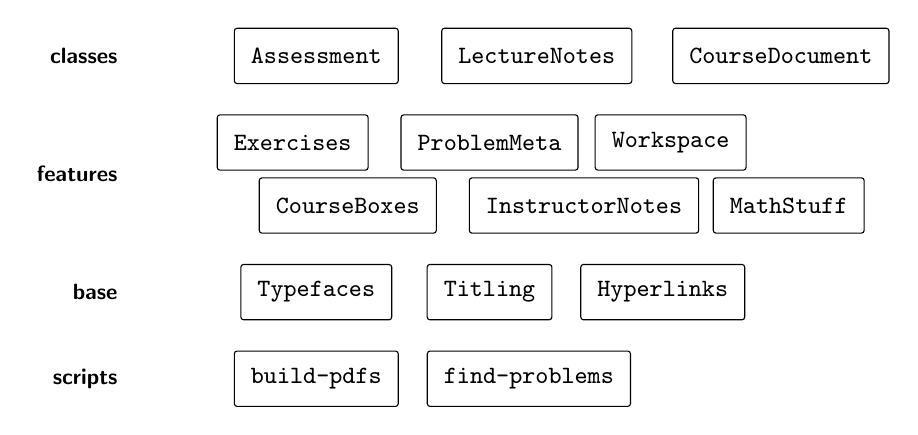
\begin{tikzpicture}[
    box/.style={draw, rounded corners=1pt, minimum height=2em,
                inner xsep=6pt, font=\small\ttfamily},
    band/.style={font=\footnotesize\sffamily\bfseries, anchor=east},
  ]
  % Row 1: the classes
  \node[band] at (-0.6, 3.1) {classes};
  \node[box] at (1.8, 3.1) {Assessment};
  \node[box] at (4.6, 3.1) {LectureNotes};
  \node[box] at (7.7, 3.1) {CourseDocument};
  % Rows 2-3: the feature packages (two rows so nothing crowds)
  \node[band] at (-0.6, 1.6) {features};
  \node[box] at (1.5, 2.0) {Exercises};
  \node[box] at (4.0, 2.0) {ProblemMeta};
  \node[box] at (6.3, 2.0) {Workspace};
  \node[box] at (2.2, 1.2) {CourseBoxes};
  \node[box] at (5.2, 1.2) {InstructorNotes};
  \node[box] at (7.8, 1.2) {MathStuff};
  % Row 4: the base
  \node[band] at (-0.6, 0.1) {base};
  \node[box] at (1.8, 0.1) {Typefaces};
  \node[box] at (4.0, 0.1) {Titling};
  \node[box] at (6.2, 0.1) {Hyperlinks};
  % Alongside: the scripts
  \node[band] at (-0.6, -1.0) {scripts};
  \node[box] at (1.8, -1.0) {build-pdfs};
  \node[box] at (4.5, -1.0) {find-problems};
\end{tikzpicture}
\end{center}

Classes pick from the features; every class stands on the base
(Assessment skips Titling and CourseBoxes; CourseDocument skips the
exercise stack). The scripts sit beside the LaTeX entirely:
\file{build-pdfs} drives latexmk and injects layer flags;
\file{find-problems} reads problem files off disk.

The honest description of the packages' relationship: \emph{not
independent, but coupled through narrow, documented contracts}. Each
package works alone or under a foreign class; where two need each other,
the seam is one macro with a fallback, or a hook with a plain default --
never a hard cross-dependency. The rest of this section documents those
seams.

\subsection{The load-order contract}\label{sec:load-order}

One ordering rule underlies every class, and Typefaces owns it:

\begin{enumerate}
  \item \textbf{amsmath before amsthm, and newtxmath loads amsthm.}
    Typefaces loads amsmath first, then newtxmath with its
    \texttt{amsthm} option -- the one point in newtxmath's load where
    amsthm can arrive in the right order. Consequently \emph{nothing else
    may load amsmath or amsthm} -- and tcolorbox drags amsmath in, which
    is why every tcolorbox-using package must come after Typefaces.
  \item \textbf{The guards enforce it.} MathStuff, CourseBoxes and
    InstructorNotes each open with a check (newtxmath or amsthm loaded?)
    and stop with a clear \cs{PackageError} naming Typefaces as the fix
    -- instead of the cryptic downstream error you would otherwise chase.
  \item \textbf{\texttt{dvipsnames} must reach xcolor first.} A class
    passes the option with \cs{PassOptionsToPackage} before anything
    loads xcolor, since xcolor's options are fixed by whoever loads it
    first.
  \item \textbf{hyperref loads last, via \cs{AtEndPreamble}.} hyperref
    patches much of LaTeX; packages loaded after it can silently undo
    those patches. Hyperlinks defers it past everything the
    \emph{document} loads too -- which \cs{AtEndPreamble} gives and
    \cs{AtEndOfClass} would not.
  \item \textbf{parskip before titlesec} (see the gotchas below for the
    failure mode).
\end{enumerate}

In practice: load Typefaces, then the feature packages, and let
Hyperlinks worry about hyperref -- the order this manual's own preamble
uses.

\subsection{Presentation hooks and narrow couplings}\label{sec:hooks}

The recurring pattern: a shared package provides the \emph{mechanism} and
a plain default look; the consuming class restyles by
\cs{renewcommand}-ing named hooks. Bookkeeping stays in the mechanism, so
no restyle can corrupt it. The instances:

\begin{itemize}
  \item \textbf{Problem headings.} A problem file names no label; the
    class does -- \cs{ProblemLabelWord}, \cs{ProblemHeadingFormat} and
    friends (section~\ref{sec:ref-exercises}) turn one environment into
    ``Problem 7.'', margin-hung ``Q7'', or a run-in ``Example.''
  \item \textbf{The label-word routing.} LectureNotes sets
    \cs{ProblemLabelWord} to read \emph{through}
    \cs{NotesProblemLabelWord}, while Assessment sets it literally to
    ``Q'' -- so a \file{course-vocab.tex} shared by both can retune the
    notes noun with no risk of renaming exam questions.
  \item \textbf{Titles and links.} \cs{TitleColor}, \cs{TitleStamp},
    \cs{LinkColor}, \cs{UrlColor}: plain defaults in the base packages,
    coloured only by CourseDocument. \cs{TitleColor} is a \emph{style}
    hook, not a colour name, precisely so Titling needs no xcolor.
  \item \textbf{\cs{WSZeroHeight}.} Exercises and InstructorNotes route
    their boxes through Workspace's overlay seam -- but each carries an
    \cs{AtBeginDocument} \cs{providecommand} identity fallback, so
    without Workspace the boxes simply render solid. One macro is the
    entire coupling.
  \item \textbf{The \cs{ProblemMeta} stub.} Exercises provides a
    swallow-the-block fallback so the essential package never depends on
    the nice-to-have one.
\end{itemize}

When you add machinery, keep the shape: mechanism $+$ default in the
shared file, look in the class, seams as single \cs{providecommand}-style
macros.

\subsection{Layers and views}

Content visibility is organised as \emph{layers}, each owned by one
package and gated by one flag: solutions and hints (Exercises),
instructor notes (InstructorNotes), the projector variant (LectureNotes).
A \emph{view} is a bundle of layers with a name and a PDF suffix, and
\file{build-pdfs} materialises it by injecting the layer definitions
before \cs{documentclass} is read (\cs{ifdefined} checks in the packages
pick them up -- no class option at any call site). The \env{instructor}
view is the maximal bundle; there is deliberately no marker tier -- the
instructor copy is the staff copy.

The overlay contract (section~\ref{sec:overlay}) is what makes the
layer model safe: turning layers on cannot move a page break, so every
view of a document is page-for-page the same paper.

\subsection{Extending the vocabulary}\label{sec:extending}

\subsubsection*{Declared numbers, and why not counters}

A theorem quoted from the course text must carry \emph{the text's}
number, but notes include only some items, so the sequence legitimately
skips. A LaTeX counter \emph{computes} numbers; a textbook number is an
external fact being \emph{mirrored} -- data, not a computation. Fighting
counters to replay someone else's sequence (scattered \cs{setcounter}s)
yields off-by-one edits and silent drift.

The mechanism that makes declaring cheap is worth recording so nobody
rediscovers it: \cs{label} never reads a counter -- it records whatever
\cs{@currentlabel} holds. So the box environments are \emph{unnumbered}
amsthm environments (\cs{newtheorem*}); the factory sets
\cs{@currentlabel} to the declared number and adds \cs{phantomsection}
for a distinct link anchor. \cs{ref} then resolves to the declared
number, and an edition change costs one token per theorem. (The same
trick, sentinel-valued, is why a stray \cs{label} on an aside prints
\texttt{[unlabelled aside]} instead of silently grabbing the section
number.)

\subsubsection*{course-vocab.tex}

The shared machinery draws a deliberate line: vocabulary every text has
(theorem, definition, \dots) and the author's own asides ship in
CourseBoxes; vocabulary \emph{specific to one text} (APEX's ``Key
Idea'', a geometry text's ``Axiom'') is declared per course, in a small
\file{course-vocab.tex} at the repo root:

\begin{manexsource}
\ifdefined\NewTextResult
  \NewTextResult[cbnote]{keyidea}{Key Idea}{cb/note}
\fi
% \renewcommand{\NotesProblemLabelWord}{Exercise}
\end{manexsource}

Masters \cs{input} it in the preamble (\cs{newtheorem} must run before
the document starts). The \cs{ifdefined} guard is what lets \emph{one}
vocab file serve every master: an Assessment document loads no
CourseBoxes, skips the factory calls, and still picks up non-box
overrides like the notes noun.

To restyle course-wide, prefer the named extension points -- the
\env{cb/*} tcolorbox styles and \env{cb*} head styles
(section~\ref{sec:ref-courseboxes}) -- over per-environment edits.

\subsubsection*{Why the exercise system is homegrown}

The obvious alternative was xsim. A usage audit of the predecessor
course showed only a narrow slice in use: numbered problem/solution
environments, a solutions toggle, points, simple layouts. The one
genuinely hard xsim feature -- \emph{body capture}, writing every
exercise out for replay elsewhere (collected solutions, exercise lists,
random pools) -- was used nowhere, and the toolkit's model is
conditional-inline (a gated \env{solution} in place), never
capture-and-replay. So the homemade system has no hidden cliff ahead:
the cliff is on a path it does not walk, and everything it does need
composes from LaTeX primitives. The trade is owning $\sim$200
understandable lines instead of vendoring $\sim$5{,}800 lines of expl3.
(No maintained alternative package exists; \file{exam.cls} is a class,
architecturally unusable inside three classes.)

\subsection{Silent-failure gotchas}\label{sec:gotchas}

The failure modes that do \emph{not} error -- collected from every
corner of the toolkit, worth a skim before debugging anything odd:

\begin{itemize}
  \item \textbf{parskip's patches fail via \cs{typeout} only.} parskip
    compensates titlesec and the TOC for paragraph skips by patching
    internals at load time; after a titlesec/amsthm upgrade a failed
    patch prints only \texttt{Couldn't patch ...} in the log. Grep for
    it: \texttt{grep "Couldn't patch" *.log}.
  \item \textbf{A reflowed \cs{ProblemMeta} block still compiles} -- and
    silently vanishes from \file{find-problems}
    (section~\ref{sec:problemmeta}).
  \item \textbf{\texttt{[5, hint]} errors} -- the lone-integer points
    shorthand works only alone; write \texttt{[points=5, hint]}.
  \item \textbf{Points are integers}; \texttt{points=2.5} errors at the
    accumulator.
  \item \textbf{\cs{printtotalpoints} and ``Page $N$ of $M$'' print
    \texttt{??} on a clean first pass} -- two-pass values; latexmk's
    rerun settles them.
  \item \textbf{\cs{label} a \env{problemgroup} inside it}, before the
    first part -- after \cs{end} it catches the last part's ``$N$(c)''.
  \item \textbf{\texttt{[unlabelled aside]} in output is the designed
    loud failure} of labelling an aside -- delete the \cs{label}.
  \item \textbf{An overlay box overprinting the content below it} is the
    leave-more-room alarm (section~\ref{sec:overlay}) -- grow the
    workspace.
  \item \textbf{\texttt{[hint]} on a hint-less file warns} rather than
    errors -- the import asked to force a hint that does not exist.
  \item \textbf{A paragraph right after \cs{FreshPage} that opens with a
    literal \texttt{[}} can be swallowed by its optional-argument scan --
    leave a blank line after \cs{FreshPage} (as you naturally would).
  \item \textbf{A \cs{workspace} at the very top of a page is discarded}
    like any top-of-page glue -- put content above it, or use
    \cs{workspace*}.
\end{itemize}

\subsection{Decoupling checklist}

The machinery still carries a little scaffolding from the course it was
built in; a final decoupling pass before any standalone handoff should:
remove the \texttt{TEMPORARY} babel/blindtext loads at the foot of
LectureNotes and CourseDocument (this manual and the demo syllabus lean
on \cs{blindtext} for filler); revisit the hardcoded
\file{~/.cache/latexmk} aux location in \file{build-pdfs}; and retarget
the source comments that still cite the private course-repo notes
(\file{NOTE.md} items) at this manual instead.


\end{document}
